\chapter{Úvod}
  Odtlačky prstov sú už vyše storočia využívané pre identifikáciu jednotlivcov vďaka unikátnemu vzoru tvoreného papilárnymi líniami na bruškách prstov.
  Takýto vzor môže slúžiť ako jedinečný podpis jednotlivca, vďaka čomu sa pôvodne odtlačky prstov začali využívať v kriminalistike. V modernm svete sa ich
  využitie značne rozšírilo a to obzvášť do osobnej autentikácie a autorizácie prístupu do zabezpečených zariadení ako sú smartfóny. Od manuálnej analýzy
  odtlačkov k automatizovanému spracovaniu však bolo potrebné vykonať výskum nielen do samotných vzorov tvorených papilárnymi líniami.
  Kapitola~{\ref{kap:odtlacok}} tejto práce je preto venovaná rôznym aspektom spojených s analýzou a spracovaním odtlačkov prstov. Je v ňej rozobraná anatómia
  kože so zameraním na oblasti, kde sa tvoria papilárne línie. Ďalej poskytuje prehľad o metódach zaznamenávania snímok štruktúr papilárnych línií od
  skenovania daktyloskopických kariet s odtlačkami prstov po moderné elektronické snímače. Posledné sekcie popisujú často využívané spôsoby spracovania
  získaných snímok a metódy analýzy štruktúr odtlačkov.

  V druhej polovici 20.~storočia sa v Spojených štátoch amerických začala digitalizácia fyzických záznamov odtlačkov prstov z dôvodu ich prudko narastajúceho
  počtu. Veľké množstvo záznamov však zabraňovalo ich digitalizácii bez kompresie, pričom ale neexistoval žiadny kompresný algoritmus, ktorý by vyhovoval
  účelom ukladania snímok odtlačkov prstov. Riešením bolo vyvinutie nového formátu, ktorý spĺňa požiadavky zachovania kvality snímok a zároveň poskytuje
  dostatočný pomer kompresie. Tento nový formát založený na diskrétnej vlnkovej transformácii bol nazvaný WSQ (angl. wavelet scalar quantization) a~vďaka
  jeho vlastnostiam kompresie sa rozšíril do väčšiny sveta. S príchodom nových skenerov vyššieho rozlíšenia však tento formát začal výkonom zaostávať a
  bolo potrebné začať využívať iný, vhodnejší formát pre ukladanie takýchto snímok. Jedným z kandidátov bol formát JPEG 2000, ktorého rentabilita v tomto smere
  sa dôkladne študovala. Formátu WSQ a jeho porovnaniu s JPEG 2000 je venovaná kapitola~{\ref{kap:wsq}}.

  Vzhľadom na množstvo rôznych úkonov spojených s analýzou odtlačkov prstov je pri študovaní týchto úkonov nápomocné mať vizuálne pomôcky
  pre demonštráciu procesov s~nimi spojených. Obrázky a náčrty v študijných materiáloch sú samozrejme veľkou pomôckou, avšak nemusia vždy
  poskytnúť tie informácie, ktoré študent potrebuje. Výstup tejto práce má za cieľ poskytnúť aplikáciu, ktorá je schopná reprodukovať
  niektoré najbežnejšie úkony predspracovania a analýzy snímok odtlačkov prstov tak, aby užívateľovi demonštrovali význam jednotlivých úkonov
  interaktívnym spôsobom na snímkach dodaných samotným užívateľom. Návrh aplikácie a jej implementácia je popísaná v kapitole~{\ref{kap:navrh_appky}}.

\chapter{Odtlačok prsta} \label{kap:odtlacok}
  Každý človek na svete je unikátne identifikovateľný podľa odtlačkov prsta. Ako prvý publikoval význam odtlačkov prstov zanechaných na miestach činu
  pre identifikáciu jednotlivcov Henry Faulds. V roku 1880 publikoval článok v žurnále \emph{Nature} informujúci výskumníkov o~jeho zisteniach o unikátnosti
  a permanencii papilárnych línii \cite{FingerprintSrcBook}. V danom článku opísal dva konkrétne prípady, kde boli využité odtlačky prstov na individualizáciu
  osôb a navrhol používanie takéhoto spôsobu identifikácie na miestach činu. V roku 1892 sir Francis Galton napísal prvú knihu o odtlačkoch
  prstov \emph{Finger Prints}, v ktorej definoval a pomenoval špecifické markanty odtlačkov prstov \cite{FingerprintSrcBook}.
  V tejto kapitole bude poskytnutý prehľad o biológii kože, klasifikácii odtlačkov prstov a o spôsoboch automatizovanej analýzy týchto odtlačkov.

  \section{Koža a jej štruktúra}
  Táto sekcia čerpala z \cite{freinkel2001skin} ak nie je uvedené inak.
  Ľudská koža je orgán obklopujúci ľudské telo plniaci mnoho účelov. Troma hlavnými účelmi kože sú ochrana pred vonkajšími vplyvmi, regulácia
  telesných charakteristík (napr. telesná teplota) a zmyslové vnímanie okolitého sveta.
  Koža sa skladá z troch hlavných vrstiev: pokožka (\emph{epidermis}), zamša (\emph{dermis}) a podkožné väzivo (\emph{hypodermis}). Tieto vrstvy sa ešte môžu
  ďalej deliť na ďalšie podvrstvy podľa účelu alebo biologického zloženia danej podvrstvy.

  \subsection{Pokožka}
  Pokožka je najvonkajšou časťou kože, ktorá je vrstvená periodicky sa regenerujúcim epitelovým tkanivom. Toto tkanivo má rôzne funkcie v rôznych
  častiach ľudského tela, pričom v prípade pokožky plní účel prevencie straty tekutín a vody, prieniku látok z vonkajšieho prostredia do tela, ale aj
  mechanickej ochrany. Táto vrstva epitelového tkaniva je \emph{avaskulárna}, čo znamená, že sa v nej nenachádzajú cievy, a teda pokožkové bunky prijímajú živiny
  najmä zo spojového tkaniva zamše.
  
  Pokožka nie je homogénna z hľadiska typov buniek v nej obsiahnutých, avšak značná väčšina (90 - 95~\% buniek) sú keratinocyty. V priebehu
  ich životného cyklu keratinocyty prejdú tzv. diferenciáciou, čo vo vývinovej biológií znamená, že bunka jedného typu (obvykle kmeňová a  málo špecializovaná)
  prejde zmenami, vďaka ktorým sa vyvinie do bunky iného typu (úzko špecializovanej bunky) \cite{slack2012biology}. Pokožku je možné deliť na ďalšie
  vrstvy znázornené na obrázku~{\ref{obr:pokozka_vrstvy}}, ktoré sú úzko spojené so štádiami diferenciácie keratinocytov. Keratinocyty sa v~pokožke vyvíjajú
  z kmeňových buniek v najhlbšej vrstve \emph{stratum basale} a počas diferenciácie migrujú k povrchu pokožky tiež nazývanou \emph{stratum corneum}. V tejto vrstve sa
  prevažne nachádzajú tzv. korneocyty, čo sú keratinocyty na konci procesu diferenciácie. Tieto bunky sú zrohovatenými keratinocytmi bez bunečného jadra
  a cytoplazmatiských organel \cite{koster2009epidermis}. Korneocyty sa následne odlupujú od pokožky pri procese deskvamácie. Celý proces migrácie
  keratinocytov po opustení \emph{stratum basale} až po \emph{stratum corneum} obyčajne trvá aspoň 14 dní, pričom deskvamácia trvá prinajmenšom ďalších 14 dní.

  \begin{figure}[h]
    \centering
    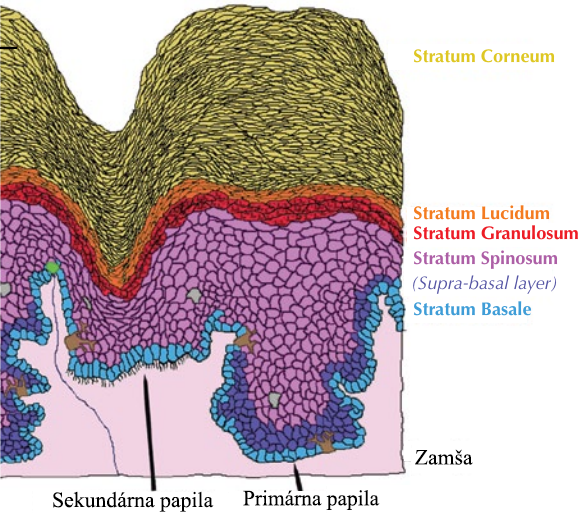
\includegraphics[width=0.65\linewidth]{obrazky-figures/pokozka_vrstvy.png}
    \caption{Vrstvy pokožky. Prevzaté z \cite{FingerprintSrcBook}.}
    \label{obr:pokozka_vrstvy}
  \end{figure}

  \subsection{Zamša}
  Pod pokožkou sa nachádza zamša, ktorá poskytuje koži jej elasticitu a pevnosť v ťahu (pevnosť materiálu pri naťahovaní). Je to spojivové tkanivo,
  a teda na rozdiel od pokožky je táto vrstva kože omnoho menej bunečná. Skladá sa hlavne z vláknitej a amorfnej medzibunkovej hmoty, pomocou ktorej dodáva
  živiny bunkám v pokožke. Hlavnými typmi vláknitého spojivového tkaniva v tejto vrstve sú kolagén a elastické spojivové väzivo, z čoho práve kolagén je
  najviac zastúpený v zamši so zastúpením približne 75~\% suchej váhy kože. Štrukturálne je zamša rozdelená na dve vrstvy - papilárna vrstva
  (\emph{stratum papilaris}) a vláknitá vrstva (\emph{stratum reticularis}).

  \textbf{Papilárna vrstva} je primárne zložená z malých zhlukov kolagénových fibríl malého priemeru a oxytalánových elastických vlákien.
  Plní úlohu spoja zamše s pokožkou. Vo volárnych (vnútorná strana ruky) a stupajových častiach kože má pokožka tvar údolí a vrchov
  (obrázok \ref{obr:zamsa_a_papily/papily_prierez}). Zamša má takýto tvar pozdĺž celej kože, aj na miestach hladkej pokožky ako je znázornené na
  obrázku~{\ref{obr:zamsa_a_papily/zamsa}}.
  Vďaka tvaru papilárnej vrstvy sa značne zvyšuje rozloha spoja medzi zamšou a pokožkou, čím sa, mimo iného, zosilňuje tento spoj.
  Týmito papilárnymi útvarmi sa prelínajú drobné krvné cievy - vlásočnice, ktoré zabezpečujú prívod živín a pomocou nich sa vykonáva aj regulácia telesnej
  teploty ich zúžením alebo rozšírením podľa potreby. V zamšových papilách sa nachádzajú aj nervové zakončenia vnímajúce externé stimuly ako sú napr. teplo a tlak.

  \textbf{Vláknitá vrstva} je oproti papilárnej zložená z kolagénových fibríl väčšieho priemeru, ktoré sa zamotávajú do veľkých zväzkov vlákien,
  okolo ktorých sa obmotávajú ďalšie elastické vlákna, čím sa značne zosilňuje ich mechanická odolnosť a pružnosť. Obecne sa tieto štruktúry zväzkov zväčšujú
  s narastajúcou hĺbkou smerom k podkožnému väzivu. V tejto vrstve sa nachádzajú vetvy autonómneho nervového systému, ktorým sa riadia telesné úkony ako potenie
  ale aj krvný tok.

  Vďaka značnému prekrveniu tejto časti kože sa tu vyskytujú mnohé iné štruktúry, jednou z ktorých sú potné žľazy. Existuje viacero typov ľudských
  potných žliaz, ako napr. \emph{apokrinné}, \emph{ekrinné} a \emph{apoekrinné}. Ďalšie delenie, hlavne apokrinných, potných žliaz je možné podľa špecializácie
  daných žliaz. Výskyt apokrinných potných žliaz je obmedzený iba na niekoľko oblastí ľudského tela. Na druhej strane sa ekrinné žľazy vyskytujú na väčšine plochy
  ľudského tela, čím sú aj najpočetnejšie pri počte dvoch až piatich miliónov žliaz. Ich účelom je primárne regulácia telesnej teploty a udržiavanie homeostázy.
  Oblasťami najhustejšieho zastúpenia týchto žliaz sú dlane a chodidlá, kde sa ich počet pohybuje okolo 2500 - 3000 na 2,5~cm\textsuperscript{2}.
  Ekrinné žľazy sú klasifikované ako jednoduché rúrkovité žľazy, ktorých vývody vyúsťujú do voľným okom neviditeľných potných pórov. Tieto póry majú
  na papilárnych valoch veľkosť približne 30~{\textmugreek{}}m. V oblastiach papilárnych valov póry sledujú priebeh papilárnych línií a objavujú sa na ich
  vrcholoch, ako je vidno na obrázku~{\ref{obr:zamsa_a_papily/papily_prierez}}.
  
  \begin{figure*}[h]\centering
    \centering
    \begin{subfigure}[b]{0.44\linewidth}
      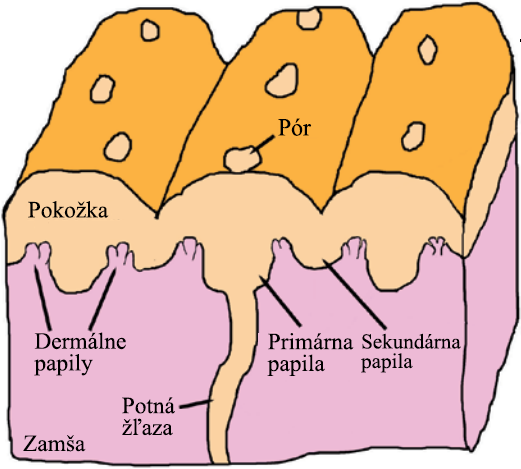
\includegraphics[width=\linewidth]{obrazky-figures/papily_prierez.png}
      \caption{}
      \label{obr:zamsa_a_papily/papily_prierez}
    \end{subfigure}
    \hfill
    \begin{subfigure}[b]{0.54\linewidth}
      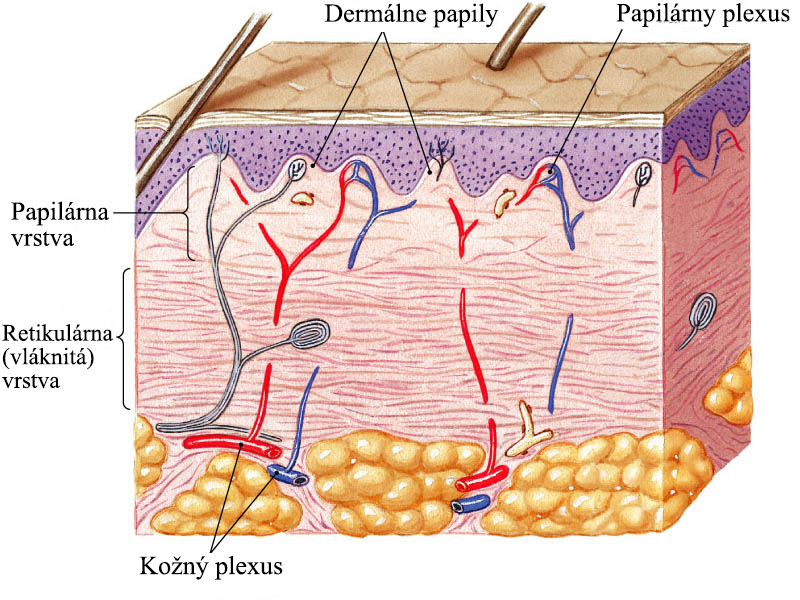
\includegraphics[width=\linewidth]{obrazky-figures/zamsa.png}
      \caption{}
      \label{obr:zamsa_a_papily/zamsa}
    \end{subfigure}
    \caption{Znázornenie štruktúr v rámci zamše.
              (a) Primárne, sekundárne a zamšové papily, prevzaté z~{\cite{FingerprintSrcBook}}.
              (b) Vrstvy a biologické štruktúry zamše, prevzaté z~{\cite{droual_dermis}}.}
    \label{obr:zamsa_a_papily}
  \end{figure*}
  
  \subsection{Podkožné väzivo}
  Pod zamšou sa nachádza podkožné väzivo zložené prevažne z tukového tkaniva, vďaka čomu nadobúda tepelnoizolačné a ochranné vlastnosti a tiež zabezpečuje
  uskladňovanie záložnej energie. Vďaka tejto vrstve má koža schopnosť sa relatívne voľne pohybovať nad hlbšími štruktúrami tela dodávajúc koži flexibilitu.
  Často do tejto vrstvy zasahujú apokrinné a~ekrinné potné žľazy a vlasové vačky s korienkami ochlpenia.

  \subsection{Papilárne línie}
  Pokožka v oblastiach dlaní a chodidiel nemá hladký povrch ako na zvyšku tela. Tieto oblasti pokožky majú valový priebeh a tvoria periodické vrcholy
  a údolia pozdĺž celej dlane a chodidla, ktoré sa nazývajú papilárne línie. Ich vlnovitý tvar dodáva pokožke pružnosť a~umožňuje pevnejšie
  uchopenie rôznych povrchov \cite{FingerprintSrcBook}.
  Pri pohľade na prierez kože na~{\ref{obr:zamsa_a_papily/papily_prierez}} je možné pozorovať prepojenie zamše s papilárnou pokožkou.
  Papilárne línie pokožky vytvárajú primárne a sekundárne výbežky zasahujúce do zamše, zvyšujúc silu spoja týchto dvoch vrstiev kože. Cez primárne výbežky
  vedú vývody ekrinných potných žliaz vyúsťujúce do pórov na vrcholoch papilárnych valov. Papilárne línie, potné žľazy
  a iné štruktúry na povrchu kože sa v následku dotyku nejakého povrchu na ňom odtlačia a zanechajú po sebe \uv{mapu},
  ktorej sa všeobecne hovorí odtlačok prsta.

  \section{Zaznamenávanie odtlačkov prsta}
  %LEFT-OFF-HERE with fixing the text based on supervisors input
  Od počiatkov identifikácie na základe papilárnych línií sa vyvinulo mnoho spôsobov zaznamenávania ich odtlačkov od prenášania odtlačku na papier
  za pomoci média ako atrament a následné skenovanie do digitálnej formy (tzv. off-line snímanie) cez optické snímanie až po termálne snímače
  (tzv. live-scan snímanie). Samotné snímanie je možné zobecniť na niekoľko krokov: senzor sníma analógové informácie o štruktúre papilárnych línií,
  ktoré sú následne konvertované do digitálnej podoby analógovo-digitálnym prevodníkom a následne sú nasnímané dáta prenesené cez komunikačné rozhranie
  na ďalšie spracovanie alebo uloženie. Nie vždy je však žiaduce snímané dáta prenášať na iný systém. V takýchto prípadoch sa využívajú čipové systémy,
  kde sa integruje snímanie a spracovanie na jednom čipe.
  V~tejto sekcii sú v krátkosti uvedené niektoré metódy snímania.

  \subsection{Optické snímače}
  Jedná sa o relatívne jednoduchý princíp snímania svetla odrazeného papilárnymi valmi. Najstaršou variantou optických snímačov je technológia \emph{FTIR}
  (Frustrated Total Internal Reflection), kde sa špička prsta položí na základňu optického hranola, pričom svetelný zdroj (obyčajne svetelná dióda) osvecuje
  papilárne valy, z čoho je pomocou zrkadlenia cez optický hranol vytvorená snímka za pomoci CCD alebo CMOS optického senzoru. Fungovanie takéhoto snímača
  je naznačené na obrázku~{\ref{obr:ftir_snimac}}. Použité osvetlenie by malo byť ploché, rozptýlené a nie priame, čím sa zabezpečí rovnomernejšie rozloženie
  svetla cez priložený prst. Vrcholy papilárnych línií, ktoré sú v kontakte s optickým hranolom, pohltia alebo rozptýlia značnú časť vyžarovaného svetla. Údolia,
  ktoré naopak nie sú v kontakte s hranolom, neovplyvňujú svetelné žiarenie, čím umožňujú svetlu odrážať sa priamo smerom k obrazovému senzoru. Vďaka týmto
  rozdielom svetelného rozptylu sa na snímači prejavia vrcholy ako tmavé a~údolia ako svetlé body na snímke. Pre koncentráciu svetla na senzor sa využíva
  optická šošovka. Existuje viacero variácií snímania založených na princípe FTIR, ktoré boli vyvinuté s účelom zmenšiť prevedenie takýchto snímačov
  pre jednoduchšiu integráciu do systémov menších rozmerov.

  \begin{figure}[h]
    \centering
    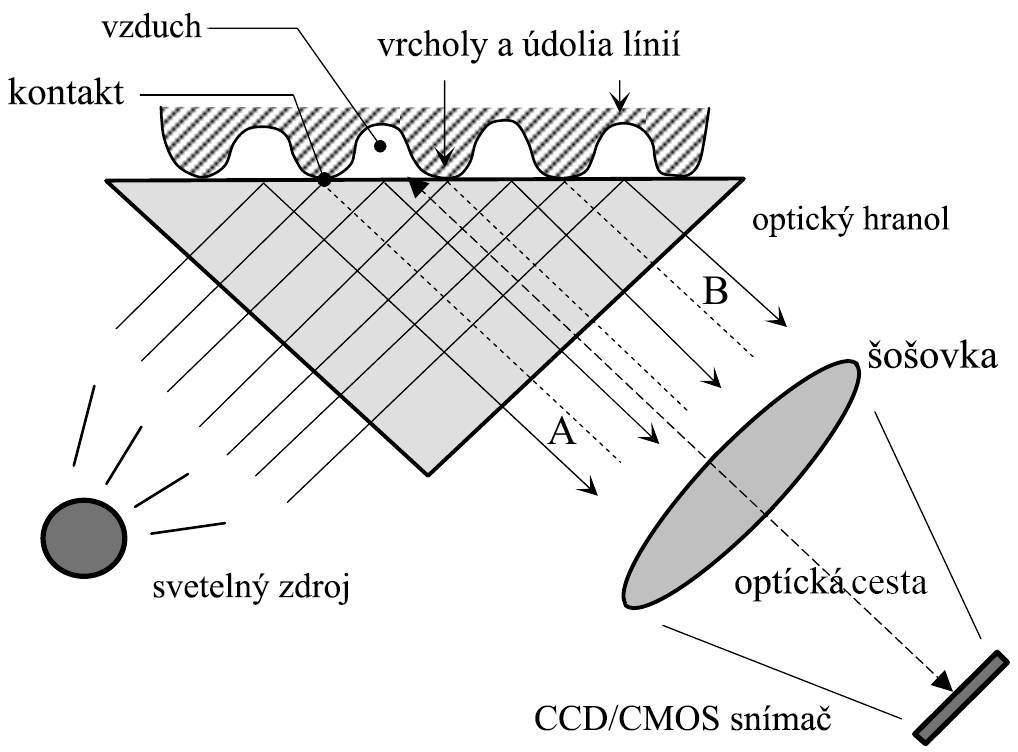
\includegraphics[width=0.6\linewidth]{obrazky-figures/ftir_snimac.png}
    \caption{Diagram znázorňujúci fungovanie FTIR snímača. Prevzaté z~{\cite{Handbook}}.}
    \label{obr:ftir_snimac}
  \end{figure}

  \subsection{Polovodičové snímače}
  Najrozšírenejším typom polovodičových snímačov sú kapacitné snímače. K rozšíreniu tohto druhu snímania prispelo rozšírenie kapacitných snímačov odtlačkov
  do väčšiny moderných smartfónov \cite{smartphone_sensors}. Kapacitné snímače odtlačkov sú založené na princípe kondenzátorov a ich schopnosti udržiavať
  elektrický náboj. Kapacitný snímač sa obecne skladá z dvoch vrstiev - izolačnej a vodivej. Izolačná vrstva sa nachádza na vonkajšej strane
  snímača, na ktorú sa položí snímaný prst. Na opačnú (vnútornú) stranu izolačnej vrstvy je naparená matica vodivých plôšok \cite{Drahansky}. Hustota týchto
  vodivých častíc musí byť vyššia, než hustota papilárnych línií kvôli zvýšeniu vzorkovacej presnosti. Pri položení prsta na snímač sa vďaka vodivosti
  pokožky a ľudského tela vytvoria malé kondenzátory tvorené prstom, izolačnou vrstvou snímača a snímacích plôšok. V týchto kondenzátoroch sa týmto vytvorí
  merateľný elektrický náboj veľkosťou závislý od vzdialenosti pokožky od náprotivných snímacích plôšok. Po~interpretácií detegovaných nábojov maticou
  snímačov je možné vytvoriť snímku odtlačku prsta.

  Medzi polovodičové snímače sa zaraďujú aj iné druhy, než kapacitné. Môže sa jednať napríklad o tepelné snímače, ktoré využívajú termoelektrické bunky
  registrujúce tepelné žiarenie papilárnych línií alebo tlakové snímače, ktoré využívajú piezoelektrický jav pre generovanie elektrického náboja
  pozdĺž papilárnych línií.

  \subsection{Ultrazvukové snímače}
  Takýto snímač pracuje na princípe vysielania ultrazvukového signálu a zaznamenávaní odrazu tohto signálu od objektov. Objektmi odrazené zvukové vlny
  majú rôzne vlastnosti v závislosti od materiálu a vzdialenosti daného objektu. Analýzou odrazeného signálu je možné vyčítať informácie o snímanom objekte,
  a to nie len v spojitosti s povrchom objektu, ale vďaka penetračným vlastnostiam zvukových vĺn aj o obsahu objektu. Týmto sa umožňuje jednoduchá detekcia
  falošných odtlačkov prstov. Pôvodne boli takéto snímače značne mechanické zariadenia s rotujúcimi ultrazvukovými vysielačmi a prijímačmi \cite{Drahansky},
  čím sa činili píliš nemotornými a drahými pre komerčné využitie. Časom sa výskum zameral na mikro-elektro-mechanické alternatívy ako
  CMUT (angl. capacitive micromachined ultrasonic transducer) \cite{savoia2010cmut} alebo PMUT (angl. piezoelectric-MUT) \cite{tang2015pmut}. Tieto technológie
  konvertujú pomocou kondenzátorov alebo piezoelektrikov striedavé napätie na zvukové vlny, čím slúžia ako ultrazvukové vysielače.

  \subsection{Zaznamenanie na fyzické médium}
  Najstarším a stále používaným spôsobom zaznamenávania odtlačkov prstov v kriminalistike je odtlačenie na fyzické médium ako je papier (daktyloskopické karty)
  pomocou špeciálneho atramentu (na Slovensku v kriminalistike nazývaný aj čerň). Takýto atrament je vyrábaný špecificky pre kriminalistické účely a má vhodné
  vlastnosti hustoty a rýchlosti sušenia pre tieto
  účely. Väčšina bežných atramentov je totiž príliš riedka alebo schne príliš pomaly, kvôli čomu sa atrament môže roztiecť a tým znehodnotiť záznam.
  V kriminalistike sa často zaznamenávajú nielen odtlačky prstov, ale celá dlaň, prípadne chodidlo - teda miesta pokožky, kde sa nachádzajú papilárne valy.

  Samotné zaznamenávanie odtlačkov prebieha prvotným nanesením tenkej vrstvy atramentu na oblasť pokožky, z ktorej sa odoberá vzorka. Nanášanie atramentu môže
  prebiehať rôzne - buď pomocou rolovania vzorkovanej časti pokožky po nanášacom pláte, ktorý je pokrytý vrstvou atramentu, alebo priamym nanesením atramentu
  nanášacím valcom. Po~aplikácií atramentu sa na daktyloskopickú kartu nanesie rolovaný odtlačok. Pri odtlačkoch prstov to znamená, že sa prst priloží
  na kartu v naklonenej polohe a prst sa roluje od jednej hrany nechta po druhú. Rolované odtlačky zaznamenávajú najväčšiu (ak nie celú) plochu pokožky
  s papilárnymi valmi, čím obsahujú veľké množstvo informácií o papilárnych líniách. Na obrázku~{\ref{obr:druhy_odtlackov}} je možné vidieť rozdiel v zaznamenanej
  ploche medzi rolovaným a~obyčajným pichaným odtlačkom. Koncom dvadsiateho storočia sa z dôvodu veľkého množstva fyzických záznamov odtlačkov vo forme
  daktyloskopických kariet začali tieto záznamy digitalizovať skenovaním. Rozšírené digitálne formáty a ich vývin sú popísané v kapitole~{\ref{kap:wsq}}.

  \begin{figure*}[h]\centering
    \centering
    \begin{subfigure}[b]{0.32\linewidth}
      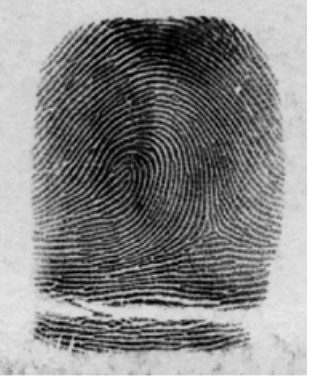
\includegraphics[width=\linewidth]{obrazky-figures/rolovany_odtlacok-Drahansky.png}
      \caption{rolovaný}
      \label{obr:rolovany_odtlacok}
    \end{subfigure}
    \hfill
    \begin{subfigure}[b]{0.32\linewidth}
      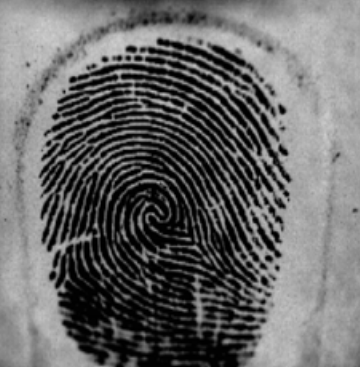
\includegraphics[width=\linewidth]{obrazky-figures/pichany_odtlacok-Drahansky.png}
      \caption{pichaný}
      \label{obr:pichany_odtlacok}
    \end{subfigure}
    \hfill
    \begin{subfigure}[b]{0.32\linewidth}
      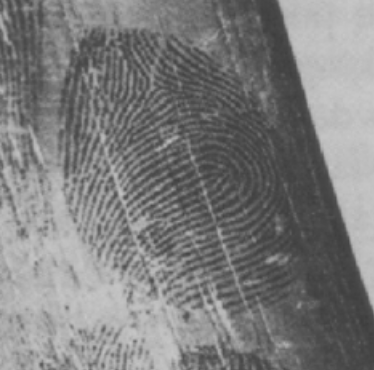
\includegraphics[width=\linewidth]{obrazky-figures/latentny_odtlacok-Drahansky.png}
      \caption{latentný}
      \label{obr:latentny_odtlacok}
    \end{subfigure}
    \caption{Rôzne typy odtlačkov prsta. V závislosti od spôsobu zanechania odtlačku je možné pozorovať rozdiely v ich kvalite a veľkosti.
            Obrázky prevzaté z~{\cite{Drahansky}}.}
    \label{obr:druhy_odtlackov}
  \end{figure*}
  
  Latentný odtlačok prsta~(\ref{obr:latentny_odtlacok}) je zastrešujúci pojem pre odtlačky prstov náhodne zanechané na povrchoch objektov, obvykle v spojitosti
  s forenznou analýzou. Pod tento pojem niektorí vyšetrovatelia zaraďujú patentné (viditeľné voľným okom), latentné (neviditeľné voľným okom) a plastické odtlačky
  (zanechané v poddajnom materiáli vytvárajúc trojrozmerný odtlačok). Pri zaznamenávaní takýchto odtlačkov sa využívajú špeciálne metódy pre ich vzorkovanie
  a zaznamenávanie (angl. fingerprint lifting).
  Pri forenznom spracúvaní latentných odtlačkov sa totiž berie na ohľad mnoho vlastností vzorkovaného odtlačku. Medzi tieto vlastnosti môže patriť aj
  chemické zloženie potu zanechaného na povrchu spolu s~odtlačkom. Podsekcia čerpala z \cite{FingerprintSrcBook}.

  Táto sekcia čerpala z \cite{Handbook} ak nie je uvedené inak.

  \section{Klasifikácia odtlačkov prstov} \label{sec:klasifikacia_odtl}
  Prvú klasifikáciu vzorov tvorených papilárnymi líniami na končekoch prstov je možné nájsť v dizertácii českého profesora Jana Evangelisty Purkyně
  z roku 1823 \cite{FingerprintSrcBook}. Začiatkom 20.~storočia Edward Henry vyvinul klasifikačný systém, ktorý bol neskôr použitý ako základ pre systém
  automatizovanej identifikácie odtlačkov prsta (AFIS). Tento systém bol vyvinutý FBI pre extrakciu markantov odtlačkov prstov automatizovanými metódami
  za pomoci počítačov. Vyvíjaný bol podľa vzoru metód a spôsobov manuálnej identifikácie, ktorú vykonávajú experti daktyloskopickej analýzy
  \cite{FingerprintSrcBook}. Tieto metódy využívajú poznatky o rôznych detailoch nachádzajúcich sa v každom zdravom papilárnom vale.
  Odtlačky prstov je možné skúmať na rôznych úrovniach detailu. Vlastne sa jedná o mieru špecifickosti, podľa akej zaraďujeme vlastnosti
  papilárnych línií na jednotlivých odtlačkoch prstov.

  \textbf{Na prvej úrovni}, najglobálnejšej, sa jedná o takzvané singularity, ktoré sa prejavujú ako náhle zmeny v priebehu papilárnych línií. Tieto 
  zmeny môžu byť časté zakončenia alebo rozdvojenia línií na malej ploche, ktoré tvoria \emph{delty} alebo ostré záhyby v líniách, 
  ktoré tvoria \emph{špirály} a \emph{slučky} definujúce \emph{jadrá} odtlačkov prstov. V praxi sa špirály bežne vynechávajú, pretože ich je možné popísať
  ako dve slučky obrátené proti sebe \cite{Handbook}. V niektorých prípadoch \cite{Drahansky, FingerprintSrcBook} sa dokonca singularity tvorené slučkami
  a špirálami zovšeobecnia iba na jadrá, pričom slučky a špirály sa rezervujú ako názvy tried odtlačkov prstov. Jadro bolo pôvodne definované Henrym \cite{Henry}
  ako \uv{najsevernejší bod najvnútornejšej papilárnej línie.}

  Obecne je na najvyššej úrovni možné každý odtlačok prsta zaradiť do tried na základe informácií o singularitách. Najrozšírenejšie triedenie odtlačkov
  prstov je triedenie podľa Henryho, ktorý definoval šesť hlavných tried podľa tvoreného obrazca papilárnymi líniami. Tieto triedy sú znázornené
  na obrázku~{\ref{obr:triedy_odtlackov}}.
  \begin{figure*}[h]\centering
    \centering
    \begin{subfigure}[b]{0.19\linewidth}
      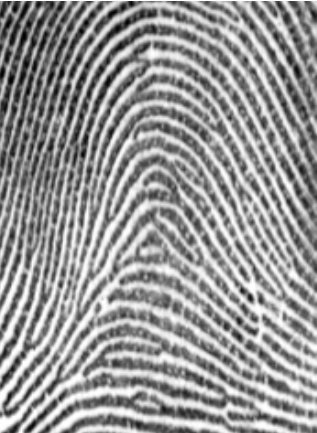
\includegraphics[width=\linewidth]{obrazky-figures/obluk.png}
      \caption{oblúk}
      \label{obr:triedy_odtlackov/obluk}
    \end{subfigure}
    \hfill
    \begin{subfigure}[b]{0.19\linewidth}
      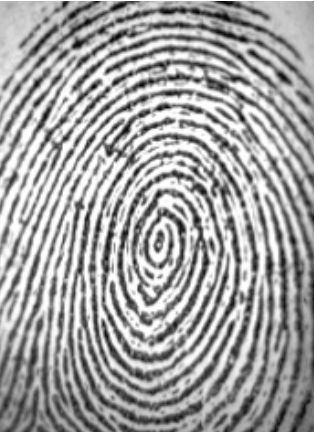
\includegraphics[width=\linewidth]{obrazky-figures/spirala.png}
      \caption{špirála}
      \label{obr:triedy_odtlackov/spirala}
    \end{subfigure}
    \hfill
    \begin{subfigure}[b]{0.19\linewidth}
      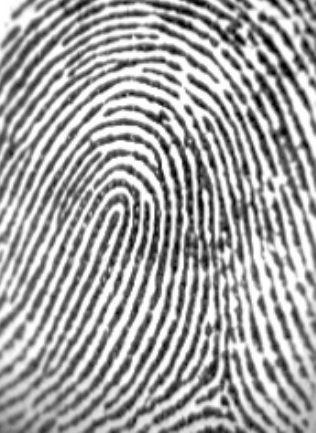
\includegraphics[width=\linewidth]{obrazky-figures/lava_slucka.png}
      \caption{ľavá slučka}
      \label{obr:triedy_odtlackov/lava_slucka}
    \end{subfigure}
    \hfill
    \begin{subfigure}[b]{0.19\linewidth}
      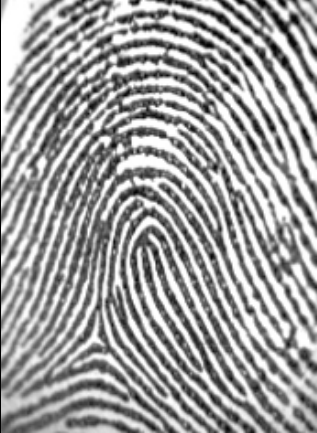
\includegraphics[width=\linewidth]{obrazky-figures/prava_slucka.png}
      \caption{pravá slučka}
      \label{obr:triedy_odtlackov/prava_slucka}
    \end{subfigure}
    \hfill
    \begin{subfigure}[b]{0.19\linewidth}
      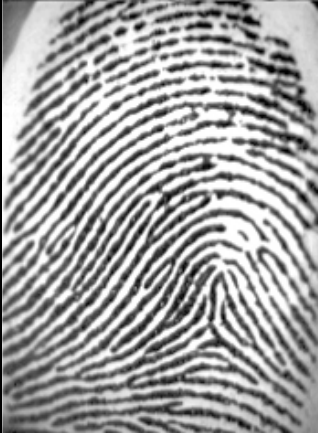
\includegraphics[width=\linewidth]{obrazky-figures/klenuty_obluk.png}
      \caption{klenutý oblúk}
      \label{obr:triedy_odtlackov/klenuty_obluk}
    \end{subfigure}
    \hfill
    \begin{subfigure}[b]{0.19\linewidth}
      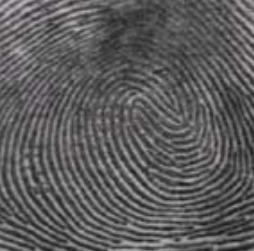
\includegraphics[width=\linewidth]{obrazky-figures/dvojita_slucka.png}
      \caption{dvojitá slučka}
      \label{obr:triedy_odtlackov/dvojita_slucka}
    \end{subfigure}
    \caption{Triedy odtlačkov prstov podľa Henryho klasifikácie \cite{Henry}. Snímky (a) až (e) prevzaté z \cite{Handbook}, (f) prevzaté z \cite{Drahansky}.}
    \label{obr:triedy_odtlackov}
  \end{figure*}
  Klasifikačný systém AFIS využívaný v FBI podľa \cite{FingerprintSrcBook} pôvodne rozlišoval prvé štyri z tried uvedených na obrázku~{\ref{obr:triedy_odtlackov}}.
  Triedy odtlačkov prsta nie sú v ľudskej populácii distribuované rovnomerne.
  Slučky majú najväčšie zastúpenie a sú pozorovateľné až u 61~\% obyvateľstva, špirály u 34~\% obyvateľstva a oblúky u zvyšných
  5~\% obyvateľstva \cite{sciencing}.

  \textbf{Na druhej úrovni}, taktiež nazývanej lokálna úroveň, pozorujeme markanty. Markanty sú útvary tvorené ukončením alebo
  vetvením papilárnych línií. Tieto útvary je možné detegovať, identifikovať a klasifikovať a následne využiť pri analýze odtlačkov prstov.
  Klasifikácia markantov je obšírnejšia, než triedenie odtlačkov prstov, pričom medzi základné markanty zaraďujeme napríklad
  ukončenie, vidličku, hák, kríženie, bočný kontakt, bod, interval, slučku, most a~priesečnú líniu \cite{Drahansky} - niektoré z nich sú znázornené na obrázku
  \ref{obr:typy_markantov}. Mnohé z vymenovaných typov majú rôzne
  variácie tvorené reťazením ich základných tvarov ako je možné vidieť na snímkach~{\ref{obr:markant_vidlicka}} a~{\ref{obr:markant_dvojita_vidlicka}}.
  Kvôli veľkému množstvu rôznych typov markantov a zložitosti ich rozlíšeniu automatizovanými systémami sa počet rozpoznávaných markantov v mnohých
  situáciách redukuje, pričom sa často využívajú iba ukončenia a vidličky.

  \begin{figure*}[h]\centering
    \centering
    \begin{subfigure}[b]{0.19\linewidth}
      
\includegraphics[width=\linewidth]{obrazky-figures/markanty/ukoncenie.png}
      \caption{ukončenie}
      \label{obr:markant_ukoncenie}
    \end{subfigure}
    \hfill
    \begin{subfigure}[b]{0.19\linewidth}
      
\includegraphics[width=\linewidth]{obrazky-figures/markanty/vidlicka.png}
      \caption{vidlička}
      \label{obr:markant_vidlicka}
    \end{subfigure}
    \hfill
    \begin{subfigure}[b]{0.19\linewidth}
      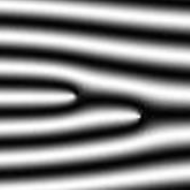
\includegraphics[width=\linewidth]{obrazky-figures/markanty/dvojita_vidlicka.png}
      \caption{dvojitá vidlička}
      \label{obr:markant_dvojita_vidlicka}
    \end{subfigure}
    \hfill
    \begin{subfigure}[b]{0.19\linewidth}
      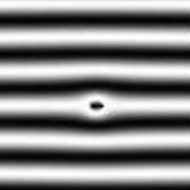
\includegraphics[width=\linewidth]{obrazky-figures/markanty/bod.png}
      \caption{bod}
      \label{obr:markant_bod}
    \end{subfigure}
    \hfill
    \begin{subfigure}[b]{0.19\linewidth}
      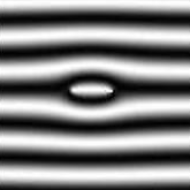
\includegraphics[width=\linewidth]{obrazky-figures/markanty/slucka.png}
      \caption{slučka}
      \label{obr:markant_slucka}
    \end{subfigure}
    \caption{Vybrané typy markantov. Čierne línie reprezentujú vrcholy papilárnych línií. Prevzaté z \cite{Drahansky}.}
    \label{obr:typy_markantov}
  \end{figure*}

  Je vhodné poznamenať, že niektoré páry markantov majú svoje inverzné náprotivky. Túto inverziu je možné vidieť na pároch~{\ref{obr:markant_ukoncenie}}
  a~{\ref{obr:markant_vidlicka}}, prípadne~{\ref{obr:markant_bod}} a~{\ref{obr:markant_slucka}}. Pri oboch pároch je možné invertovať
  hodnoty šedej v snímke a výsledné markanty klasifikovať opačne ako pri originálnych snímkach. Takáto nejednoznačnosť môže spôsobiť problémy pri porovnávaní
  rôznych odtlačkov prstov aj od tej istej osoby, pretože takáto inverzia môže nastať aj pri snímaní odtlačku v dôsledku rôzne aplikovaného tlaku počas
  zaznamenávania odtlačku. Aj z tohto dôvodu sa zaznamenávajú nielen polohy daných markantov, ale aj uhol zvieraný smerom markantu a horizontálnej osi
  snímky, ktorý zostane rovnaký aj pri inverzií z vidličky na ukončenie alebo naopak \cite{Handbook}.

  \textbf{Na tretej úrovni}, najlokálnejšej, sa rozoznávajú detaily kože a atribúty papilárnych línií. Na tejto úrovni je možné pozorovať
  póry, šírku papilárnych línií, jazvy a poranenia kože, kožné ochorenia, atp. Dlhú dobu sa pri automatizovanej analýze detaily na tejto úrovni
  nespracúvali z dôvodu, že pri nižších rozlíšeniach snímok, typicky pod 1000 ppi (bodov na palec - jednotka používaná napr. pri snímačoch a skeneroch),
  tieto detaily nie sú spoľahlivo pozorovateľné \cite{Handbook}. Vylepšovaním snímačov odtlačkov sa však otvorili možnosti detekcie pórov a na ich základe
  zvyšovanie spoľahlivosti porovnávania odtlačkov prstov automatizovanými systémami.

  Jeden z prvých návrhov automatického autentizačného systému pracujúceho s detailmi tretej úrovne uviedli Stosz a Alyea \cite{StoszAlyea}, ktorí predviedli
  uskutočniteľnosť ich návrhu zabezpečením počítača takýmto systémom.
  V roku 2006 Jain, Chen a Demirkus \cite{jain2006pores} predstavili porovnávanie odtlačkov prstov na základe rozšírenia typického porovnávania
  podľa prvých dvoch úrovní detailu o póry z tretej úrovne. Ich metóda spočíva na dvoj-krokovom rozpoznávaní. Najprv podľa detailov druhej úrovne (markantov)
  natočia vstupné snímky tak, aby mali zhodnú orientáciu a následne vygenerujú spoločné hodnotenie zhody podľa druhej a tretej úrovne detailu na výreze odtlačku.
  Úspešnosť detekcie zhody bola podľa ich zistení touto metódou zvýšená. Ich zistenia tým podporili koncept využívania detailov tretej úrovne pri
  automatizovanej analýze a to obzvlášť pre odtlačky, resp. časti odtlačkov prstov, kde sa nenachádza veľké množstvo informácií obsiahnutých na
  nižších úrovniach detailu.

  \section{Spracovanie a analýza snímok odtlačkov prstov} \label{sec:analyza}
  %V súčasnosti automatizované analyzátory odtlačkov prstov vyžadujú úpravu zdrojových snímok. Surové snímky odtlačkov totiž nie sú vhodné pre
  %extrakciu informácí pomocou algoritmov. Skôr, než sa zo snímok môžu začať extrahovať vlastnosti ako singularity a markanty je potrebné snímku
  %spracovať tak, aby sa so snímkou pracovalo jednoduchšie pri samotnej analýze.

  %Medzi hlavné kroky spracovania vstupnej snímky patria zníženie šumu snímky, zvýšenie kontrastu a binarizácia snímky a ztenšenie línií.

  Metódy spracovania a analýzy odtlačkov prstov sa líšia na základe požadovanej aplikácie analyzátora. Napríklad pri zabezpečovaní mobilných telefónov
  sa nekladie až taký dôraz na kvalitu analýzy ako napríklad v kriminalistike, a teda sa mnohé časti analýzy preskočia, prípadne
  sa im nevenuje veľká pozornosť za účelom zrýchlenia systému. Avšak hlavná kostra analýzy je vždy relatívne nemenná.

  % //TODO: mozno nejaky obrazok o process flow pri spracovani a analyze pre ilustraciu poradia ukonov

  \subsection{Vylepšenie snímok} \label{sec:vylepsenie_snimok}
  Jedným z prvých krokov spracovávania snímok odtlačkov prstov je ich vylepšenie (angl. image enhancement). Väčšina zdrojov odtlačkov je nespoľahlivých
  v zmysle, že nie je možné zaistiť aby boli zdrojové snímky bez signálového alebo iného šumu. To platí hlavne v kriminalistike,
  kde sa často pracuje s latentnými odtlačkami nízkej kvality. Z tohto dôvodu je dôležité vstupnú snímku nejakým spôsobom upraviť tak,
  aby dopad šumu prítomného v snímke a prípadne chýbajúcich alebo narušených častí odtlačku bol minimalizovaný v neskorších krokoch spracovania,
  napríklad pri extrakcii markantov.

  Snímky odtlačkov, prípadne ich oblasti je možné zaradiť do troch kategórii na základe kvality a rozoznateľnosti papilárnych línií:
  \begin{itemize}
    \item \emph{Dobre rozoznateľná oblasť} obsahuje jasne oddelené hrebene od údolí papilárnych línií bez prerušení ich priebehu.
    \item \emph{Poškodená zotaviteľná oblasť} obsahuje malé množstvo narušení priebehu línií ako sú napríklad drobné jazvy, mierne poškodenie
          samotného odtlačku apod., avšak snímka je stále dostatočne jednotná aby z nej bolo možné extrahovať užitočné informácie.
    \item \emph{Poškodená nezotaviteľná oblasť} je oblasť, ktorá je natoľko poškodená, že extrakcia informácií o štruktúrach papilárnych línií
          z nej nemá zmysel \cite{Hong}.
  \end{itemize}
  Operácie vylepšenia snímok majú za úlohu zvýšiť rozoznateľnosť priebehu papilárnych línií v prvých dvoch kategóriách a odstrániť oblasti tretej
  kategórie \cite{Hong}.
  
  Kroky vedúce k vylepšenej snímke však nie sú striktne obmedzené na redukciu šumu. Zvýšenie kontrastu medzi papilárnymi líniami a údoliami medzi nimi
  je taktiež kľúčová k neskorším úpravám snímky.

  \subsubsection{Normalizácia} \label{sec:normalizacia}
  Jedným z prvých krokov predspracovania vstupnej snímky odtlačku prstu je normalizácia. Jedná sa o operáciu, ktorá má za cieľ znížiť variácie
  v hodnotách odtieňov šedej, čím sa podporí kvalitnejší výstup ďalších krokov spracovania \cite{Hong}. Jedným zo spôsobov ako normalizovať
  snímku je upraviť variáciu a strednú hodnotu snímky pomocou vzorca~{\ref{eq:normalizacia_Hong}}.

  \begin{equation}
    G(i,j) =
    \begin{cases}
      M_0 + \sqrt{\frac{V_0 (I(i,j)-M)^2}{V}}  & \text{ak } I(i,j) > M \\
      M_0 - \sqrt{\frac{V_0 (I(i,j)-M)^2}{V}} & \text{inak,}
    \end{cases}
    \label{eq:normalizacia_Hong}
  \end{equation}
  kde $I(i,j)$ je pixel originálnej snímky, $G(i,j)$ je pixel normalizovanej snímky, $M$ je stredná hodnota snímky a $V$ je variácia (rozptyl) hodnôt snímky.
  Hodnoty $V_0$ a $M_0$ sú hodnoty požadovanej variácie a strednej hodnoty normalizovanej snímky, ktoré Hong definuje ako $V_0 = M_0 = 100$ \cite{Hong}.

  Ďalšou možnosťou normalizácie je vyrovnanie histogramu. Táto úprava má dopad na zlepšenie kontrastu pri nadmerne tmavých
  alebo nadmerne bledých snímkach. Vyrovnanie intenzít jednotlivých odtieňov šedej má za účinok zvýšenie kontrastu v hmlistej zdrojovej snímke.
  Metódy ekvalizácie histogramu však môžu nežiadúco zvýrazniť šum obsiahnutý v snímke. Z tohto dôvodu sú často využívané modifikované metódy,
  ako napríklad adaptívna ekvalizácia histogramu, v spojení s filtrom.

  \subsection{Oblasť záujmu}
  Ako bolo spomenuté v úvode do sekcie~{\ref{sec:vylepsenie_snimok}}, odtlačky prsta môžu obsahovať nezotaviteľné oblasti, ktoré žiadnym významným spôsobom
  neprispievajú k analýze samotného odtlačku. Okrem toho snímky odtlačkov prstov obsahujú aj tzv. pozadie, čo je v kontexte snímok odtlačkov prstov oblasť,
  ktorá neobsahuje odtlačok papilárnych línií prsta. Pri analýze odtlačkov prsta je tým pádom vhodné takéto časti snímky maskovať a ponechať iba takzvanú
  oblasť záujmu (angl. region of interest). Takéto maskovanie môže mať významný dopad na rýchlosť algoritmov aplikovaných v ďalších krokoch spracovania,
  pretože maskované oblasti je možné ignorovať.

  Jedným z najzákladnejších prístupov k vytvoreniu masky oblasti záujmu je jednoduchá analýza rozptylu hodnôt pixelov v rámci blokov snímky. Je to elegantné
  riešenie, pretože v mnohých prípadoch sú nezotaviteľné oblasti, podobne ako pozadie, oblasťami nízkeho rozptylu hodnôt - a to či už nízkych hodnôt, v prípade
  tmavých častí odtlačku v dôsledku nadmerného tlaku pri získavaní odtlačku, alebo vysokých hodnôt, ktoré sú vytvárané napríklad z dôvodu ochorenia kože.
  Analýza prebieha tak, že sa snímka rozdelí na bloky veľkosti $w\times{}h$ a pre každý z týchto blokov sa vypočíta priemerný rozptyl na základe vzorcov
  \begin{equation}
    V(b) = \frac{1}{wh} \sum_{i=1}^{w}\sum_{j=1}^{h}(I(i,j) - M(b))^2
  \end{equation}
  \begin{equation}
    M(b) = \frac{1}{wh} \sum_{k=1}^{w}\sum_{l=1}^{h}(I(k,l)),
  \end{equation}
  kde $b$ je blok pixelov s rozmermi $w\times{}h$ a $I$ je vstupná snímka odtlačku prsta. Funkcia $M(b)$ teda počíta priemernú hodnotu v rámci bloku $b$
  a funkcia $V(b)$ rozptyl hodnôt v~bloku~{$b$}~{\cite{babatunde2012FP_enhancement}}. V prípade, že rozptyl v bloku je nad istou prahovou hranicou, jedná sa
  o oblasť záujmu, inak sa jedná o pozadie. Takýto algoritmus je možné aplikovať rôznymi spôsobmi, a to napríklad po pixeloch, kde je výpočet rozptylu
  aplikovaný na oblasť okolo každého pixelu a pixely sa maskujú jednotlivo, alebo po častiach, kde sa maskuje celý blok a okno pre výpočet rozptylu sa
  posúva o viac, než jeden pixel.

  \begin{figure}[h]
    \centering
    \begin{subfigure}[b]{0.3\linewidth}
      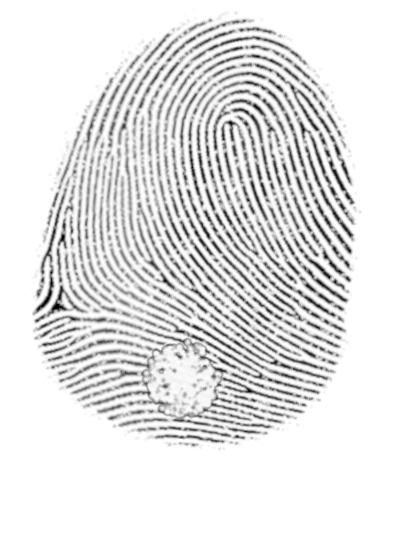
\includegraphics[width=\linewidth]{obrazky-figures/roi_template.png}
      \caption{pôvodná snímka}
      \label{obr:roi_template}
    \end{subfigure}
    \hfill
    \begin{subfigure}[b]{0.3\linewidth}
      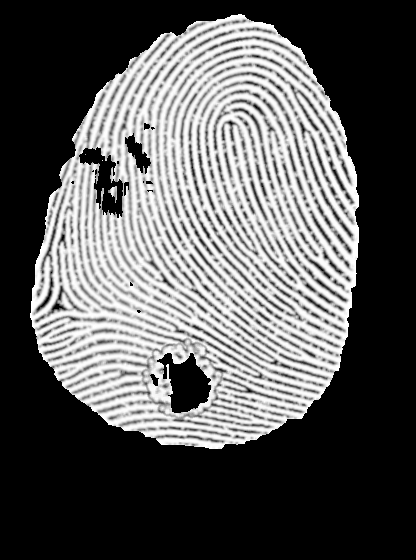
\includegraphics[width=\linewidth]{obrazky-figures/roi_pixel-wise.png}
      \caption{pixelová maska}
      \label{obr:roi_pixel-wise}
    \end{subfigure}
    \hfill
    \begin{subfigure}[b]{0.3\linewidth}
      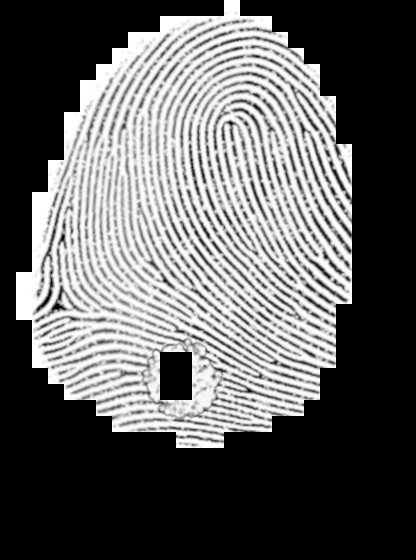
\includegraphics[width=\linewidth]{obrazky-figures/roi_block-wise.png}
      \caption{bloková maska}
      \label{obr:roi_block-wise}
    \end{subfigure}
    \caption{Zobrazenie prístupu aplikácie masky po pixeloch a po blokoch na snímke syntetického odtlačku prsta s nezotaviteľnou oblasťou.
            Snímka z internej databázy STRaDe.}
    \label{obr:typy_roi_masiek}
  \end{figure}

  Na obrázku~{\ref{obr:typy_roi_masiek}} je možné vidieť rozdiel medzi dvoma uvedenými spôsobmi aplikácie masky pri rovnakej prahovej hodnote.
  Ako je vidno, maskovanie po pixeloch produkuje presnejšiu masku v okolí pozadia a nezotaviteľnej časti snímky. Avšak produkuje aj nesprávne časti masky,
  ako je vidno v pravej hornej časti snímky~{\ref{obr:roi_pixel-wise}}. Úpravou prahovej hodnoty je možné predísť takýmto falošným detekciám, ale obecne z mojich
  pozorovaní môžem uviesť, že aplikácia masky po blokoch je robustnejšia, pričom však produkuje nepresnejšiu masku.
  
  \subsection{Orientácia} \label{sec:orientacia}
  Lokálna orientácia papilárnych línií v snímke je uhol zvieraný líniami v jej lokalizovanej časti okolo daného bodu
  s horizontálnou osou snímky. Konkrétnejšie, je to uhol zvieraný líniami v ľubovoľnej oblasti okolo pixelu $[x,y]$ s
  horizontálnou osou snímky. Pri automatizovanej analýze sa často orientácia neprepočítava pre každý pixel z dôvodu zníženia času predspracovania snímky.
  Namiesto toho je možné ju vypočítať diskrétne pre časti snímky a následne interpoláciou takto získaných orientácií je možné aproximovať
  orientáciu papilárnych línií v okolí explicitne vyhodnotenej časti snímky \cite{Handbook}.

  Orientáciu línií je možné vypočítať mnohými spôsobmi, v tejto práci sa však venujem metóde navrhnutej Hongom et al. v \cite{Hong}.
  Táto metóda sa spolieha na výpočet gradientu Sobelovým, prípadne obdobným operátorom. Postup výpočtu je nasledovný:
  \begin{itemize}
    \item Vstupná snímka sa rozdelí na $h \times w$ bloky
    \item Vypočíta sa gradient Sobelovým operátorom
    \item Odhadne sa lokálna orientácia bloku pomocou rovníc:
          \begin{equation}
            \mathcal{V}_x(i,j) = \sum_{u=i-\frac{h}{2}}^{i+\frac{h}{2}}\sum_{v=j-\frac{w}{2}}^{j+\frac{w}{2}} 2\partial _{x}(u,v) \partial _y(u,v),
          \end{equation}
          \begin{equation}
            \mathcal{V}_y(i,j) = \sum_{u=i-\frac{h}{2}}^{i+\frac{h}{2}}\sum_{v=j-\frac{w}{2}}^{j+\frac{w}{2}} (2\partial ^{2}_{x}(u,v) - \partial ^{2}_{y}(u,v)),
          \end{equation}
          \begin{equation}
            \theta{}(i,j) = \frac{1}{2}\tan{}^{-1}(\frac{\mathcal{V}_y(i,j)}{\mathcal{V}_x(i,j)}),
          \end{equation}
          kde $\theta{}(i,j)$ je aproximáciou lokálnej orientácie línií metódou najmenších štvorcov pre blok so stredom na pixeli $(i,j)$. Premenné
          $\partial _{x}$ a $\partial _{y}$ sú dvojrozmerné polia obsahujúce vypočítaný gradient v príslušných smeroch, $u$ a $v$ reprezentujú indexy v rámci
          výpočtového bloku $h \times w$.
  \end{itemize}

  \subsection{Frekvencia papilárnych línií}
  Dôležitým krokom, obzvlášť pred následnou úpravou vstupnej snímky filtrom závislým na frekvencii papilárnych línií, je výpočet ich lokálnej frekvencie.
  Frekvenciu papilárnych línií v~nejakom bode $[i,j]$ je možné definovať ako počet vrcholov pozdĺž výrezu so stredom v danom bode $[i,j]$,
  ktorý je kolmý na lokálnu orientáciu línií $\theta_{ij}$. Frekvencia sa obyčajne počíta pre každý bod, alebo pre malé diskrétne bloky snímky odtlačku prsta,
  pretože hustota vrcholov papilárnych línií sa môže líšiť aj v rámci jedného prsta \cite{Handbook}.

  Existuje viacero prístupov k odhadnutiu frekvencie vrcholov papilárnych valov. Jednou z nich je metóda navrhnutá Hongom et al. v \cite{Hong} (zobrazená na
  obrázku~{\ref{obr:frekvencia-Hong}}),
  ktorá priamo analyzuje odtiene šedej a ich priebeh v originálnej snímke. Táto metóda priamo aplikuje vyššie uvedenú definíciu na snímku nasledovne:

  \begin{enumerate}
    \item Okno veľkosti $l \times{} w$ sa vytvorí okolo pixelu $[i,j]$. Toto okno je natočené kolmo na smer priebehu papilárnych línií.
    \item Vypočíta sa $x$-signatúra $X$ spriemerovaním hodnôt pixelov pozdĺž stĺpcov $l$ orientovaného okna.
    \item V prípade, že v orientovanom okne sa nenachádzajú markanty alebo singulárne body, je získaná $x$-signatúra formou sínusová. Vďaka tomu je
          možné frekvenciu medzi vrcholmi vypočítať ako inverziu priemerného počtu pixelov medzi jednotlivými vrcholmi papilárnych línií.
  \end{enumerate}
  Papilárne línie však nemajú uniformný priebeh naprieč celým odtlačkom. V takýchto prípadoch, keď sa v orientovanom okne nachádzajú oblasti, ktoré narúšajú
  hladký sínusový priebeh línií, Hong aplikuje interpoláciu frekvencií z okolitých blokov snímky, čím aproximuje frekvenciu pre danú oblasť. Hong taktiež uvádza
  priemernú frekvenciu línií medzi hodnotami $1/3$ a $1/25$, na základe ktorých prahuje vypočítané frekvencie na platné a neplatné.

  \begin{figure}[h]
    \centering
    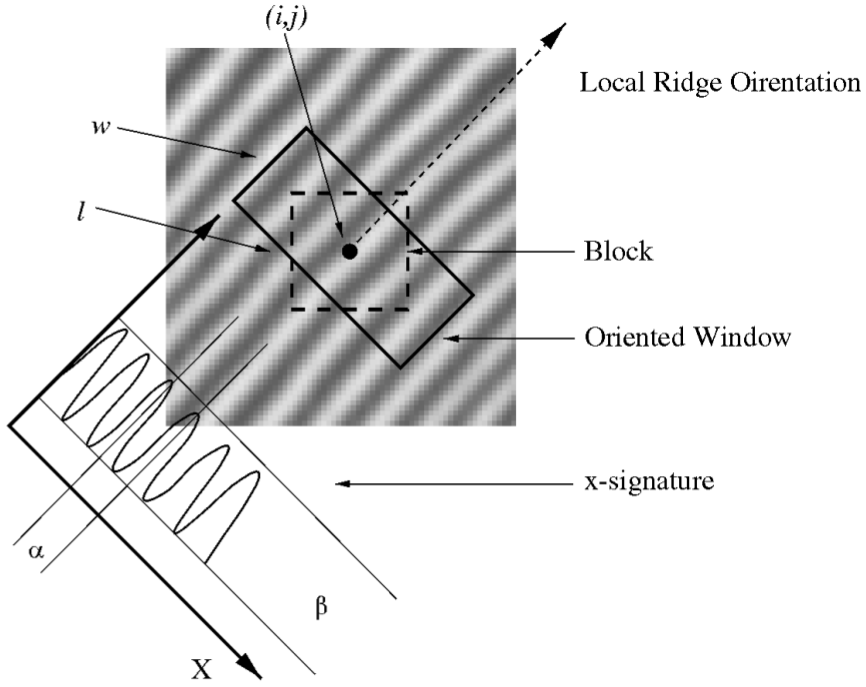
\includegraphics[width=0.7\linewidth]{obrazky-figures/frekvencia-Hong.png}
    \caption{Orientované okno naprieč papilárnymi líniami a ich $x$-signatúra. Prevzaté z \cite{Hong}.}
    \label{obr:frekvencia-Hong}
  \end{figure}

  \subsection{Gaborova funkcia}
  Gaborova funkcia je využívaná pre zvýšenie kvality snímok znížením šumu v snímke a zachovaním štruktúry papilárnych línií. Jedná sa o kontextuálny
  filter, ktorý na rozdiel od iných konvolučných filtrov filtruje na základe lokálnych informácií o snímke \cite{Handbook}. Gabor filter je vhodný
  pre filtrovanie snímok odtlačkov, pretože zdieľa isté vlastnosti ich dvojrozmernej reprezentácie. Týmito vlastnosťami sú orientácia a frekvencia,
  ktoré je možné extrahovať zo snímky odtlačku prsta. Vďaka týmto zdieľaným vlastnostiam je možné pre každý pixel snímky vygenerovať prispôsobený konvolučný
  filter, čím sa redukuje, prípadne úplne zamedzuje, používaniu preddefinovaných filtrov obmedzeného počtu. V prípade využitia preddefinovaných filtrov je totiž
  nutné využiť najlepšiu zhodu filtra s konkrétnou orientáciou a frekvenciou v danom bode snímky, čím sa zhoršujú výsledky filtrovania.
  Na obrázku~{\ref{obr:gabor_kernel}} je zobrazené konvolučné jadro Gabor filtra vygenerované v programe
  \mbox{MATLAB}\footnote{\url{https://www.mathworks.com/products/matlab.html}}.
  
  \begin{figure}[h]
    \centering
    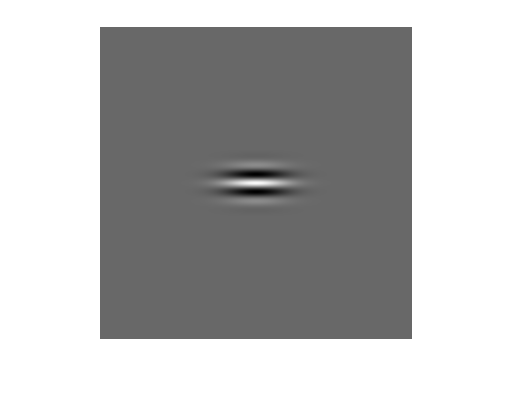
\includegraphics[width=0.25\linewidth]{obrazky-figures/gabor_kernel.png}
    \caption{Príklad jadra (angl. kernel) Gabor filtra vytvorený v programe MATLAB s parametrami $f = 20$pixelov/cyklus a $\phi{} = 0$ radiánov.}
    \label{obr:gabor_kernel}
  \end{figure}
  Matematický zápis Gabor filtra je nasledovný:
  \begin{equation}
    h(x,y: \phi{}, f) = \exp{\left\{ -\frac{1}{2} \left( \frac{x_\phi{}^2}{\delta{}_x^2} \right) + \left( \frac{y_\phi{}^2}{\delta{}_y^2} \right) \right\}} \cos{}\left(2\pi{}fx_\phi{}\right),
  \end{equation}
  kde $\phi{}$ je orientácia a $f$ je frekvencia pixelu, na ktorom sa vykonáva operácia konvolúcie. Hong definuje $\delta{}_x$ a $\delta{}_y$
  ako konštanty s hodnotou 4 na základe pozorovaní \cite{Hong}. Samotné filtrovanie je konvolúciou každého pixelu snímky odtlačku prsta s vygenerovaným filtrom
  pre daný pixel. Veľkosť konvolučného jadra Gabor filtra Hong definuje v oboch smeroch na $k = 11$ pixelov.

  \subsection{Binarizácia}
  Adaptívna binarizácia podľa Bradleyho \cite{bradley2007adaptive} je jednou z využívaných binarizačných algoritmov pri analýze odtlačkov prstov.
  Metóda využíva priemer hodnôt v okne $s \times s$ v okolí každého pixelu snímky. Tento priemer je získaný pomocou integrálneho obrazu, ktorý je pred-počítaný
  z pôvodnej snímky. Následne sa získaný priemer prahuje cez hodnotu $t$, ktorá definuje, o koľko percent môže byť súčasný pixel nižší, než lokálny priemer.
  Teda, ak má súčasný pixel o {$t$}~\% nižšiu hodnotu, než okolie, je nastavený na čiernu, inak je to biely pixel. Výhodou takéhoto prahovania hodnôt oproti
  globálnemu prahu, ktorý sa aplikuje na celú snímku je, že sa prispôsobuje oblastiam snímky v závislosti od kontrastu, resp. od rozptylu hodnôt v okolí
  súčasne spracovávaného pixelu.

  \subsection{Stenčovanie línií}
  Tento krok sa vykonáva na binarizovaných snímkach odtlačkov. Jedná sa o stenčenie línií tvorených odtlačkom prsta na čiernobielej snímke na šírku
  jeden pixel. Týmto sa uľahčuje strojová analýza markantov a singularít, pretože po stenčení je možné pracovať iba s \emph{kostrou} odtlačku,
  ktorá obsahuje iba priebeh papilárnych línií vrátane bodov záujmu ako sú spomenuté markanty, ktoré nezávisia na hrúbke línií.
  Metódy extrakcie markantov, vrátane extrakcie z obrázkov so stenčenými líniami sú v sekcii~{\ref{sec:analyza_markantov}}.
  
  Extrakcia stenčenej kostry binárnej snímky zohráva významnú rolu v oblasti rozpoznávanie tvarov (angl. pattern recognition). Obzvlášť veľké využitie má stále
  pri počítačovom videní (rozpoznávanie písma alebo rôznych tvarov), napriek tomu, že v tejto oblasti sa rýchlo rozširuje umelá inteligencia.
  Samotné stenčovanie však môže do extrahovanej kostry snímky zaviesť falošné \uv{výrastky} z dôvodu nerovnomernosti línií v pôvodnej snímke.
  Pri analýze odtlačkov prsta má stenčovanie vzorov papilárnych línií význam pre extrakcii markantov. Znamená to, že kvalitne stenčené línie zvyšujú kvalitu
  extrakcie markantov. Prístupov k zvýšeniu kvality stenčených línií je viacero, ako napríklad vypĺňanie menších dier v líniách alebo normalizácia šírky
  línií na konštantnú šírku pomocou filtrov \cite{Handbook}. Jedným z~prístupov je aj využiť algoritmus stenčovania, ktorý bol navrhnutý s úmyslom zredukovať
  falošné výbežky v kostre. Jedným z takýchto algoritmov je Zhang-Suen \cite{ZhangSuen_thinning}, ktorý mal za cieľ minimalizovať tvorbu falošných výrastkov
  a zároveň maximalizovať rýchlosť procesu stenčovania.
  
  \begin{figure}[h]
    \centering
      \begin{tabular}{ l | c | c | c | l }
        \multicolumn{5}{c}{sever} \\
        \cline{2-4}
        & \makecell{$P_9$ \\ $[i-1,j-1]$} & \makecell{$P_2$ \\ $[i-1,j]$} & \makecell{$P_3$ \\ $[i-1,j+1]$} \\ \cline{2-4}
        západ & \makecell{$P_8$ \\ $[i,j-1]$} & \makecell{$P_1$ \\ $[i,j]$} & \makecell{$P_4$ \\ $[i,j+1]$} & východ \\ \cline{2-4}
        & \makecell{$P_7$ \\ $[i+1,j-1]$} & \makecell{$P_6$ \\ $[i+1,j]$} & \makecell{$P_5$ \\ $[i+1,j+1]$} \\
        \cline{2-4}
        \multicolumn{5}{c}{juh}
      \end{tabular}
    \caption{Okolie pixelu $[i,j]$ (označený $P_1$) v binárnej snímke $I$. Prevzaté z \cite{ZhangSuen_thinning}.}
    \label{obr:okolie_ZhangSuen}
  \end{figure}

  Jedná sa o paralelný algoritmus, ktorý definuje výstupný pixel $[i,j]$ binárnej snímky $I$ ako funkciu jeho okamžitého okolia. Pixely patriace kostre
  pôvodnej snímky majú hodnotu~1, pričom pozadie má hodnotu~0. Okolie pixelu, na základe ktorého je uvedené rozhodnutie, či bude daný pixel vymazaný z kostry,
  má veľkosť $3 \times 3$ a definuje kruhový orientovaný sled pixelov (zobrazené na~{\ref{obr:okolie_ZhangSuen}}).
  Každá iterácia algoritmu je rozdelená na dve poditerácie. Význam tohto rozdelenia je v zachovaní spojitého priebehu kostry pôvodnej snímky.
  V~každej z poditerácii sa skontrolujú podmienky pre odstránenie daného pixelu:
  \begin{enumerate}
    \item Prvá poditerácia \label{itm:thin_step_1}
    \begin{enumerate}
      \item $A(P_1) = 1$  \label{itm:thin_step_1a}
      \item $2 \leq B(P_1) \leq 6$ \label{itm:thin_step_1b}
      \item $P_2 * P_4 * P_6 = 0$ \label{itm:thin_step_1c}
      \item $P_4 * P_6 * P_8 = 0$ \label{itm:thin_step_1d}
    \end{enumerate}
    \item Druhá poditerácia \label{itm:thin_step_2}
    \begin{enumerate}
      \item \emph{identická ako prvá podmienka prvej poditerácie} \label{itm:thin_step_2a}
      \item \emph{identická ako druhá podmienka prvej poditerácie} \label{itm:thin_step_2b}
      \item $P_2 * P_4 * P_8 = 0$ \label{itm:thin_step_2c}
      \item $P_2 * P_6 * P_8 = 0$. \label{itm:thin_step_2d}
    \end{enumerate}
  \end{enumerate}

  Prvý krok oboch poditerácii definuje funkciu $A(P_1)$, ktorá vracia počet prechodov z~pixelu hodnoty 0 na pixel hodnoty 1 v kruhovom orientovanom slede
  pixelov $P_2\dots{}P_9$ okolo pixelu $P_1$. Týmto sa predíde odstráneniu pixelu uprostred kostry línie medzi dvoma koncovými bodmi.
  Funkcia $B(P_1)$ vracia počet nenulových pixelov v slede pixelov $P_2\dots{}P_9$. Táto podmienka zachováva koncové body
  kostry. Posledné dve podmienky oboch poditerácií kontrolujú, či je daný pixel hraničným pixelom medzi kostrou a pozadím.
  Napríklad podmienky~{\ref{itm:thin_step_2c}} a~{\ref{itm:thin_step_2d}} kontrolujú hraničné pixely na severe a západe kostry a juho-východné rohové pixely
  kostry. V prípade, že sú splnené všetky podmienky, pixel $[i,j]$ je vymazaný (resp. prepísaný na hodnotu 0), inak zostáva nezmenený \cite{ZhangSuen_thinning}.

  \section{Spôsoby analýzy markantov} \label{sec:analyza_markantov}
  Detaily druhej úrovne na odtlačkoch prstov poskytujú veľmi robustné, počítačom analyzovateľné, identifikačné informácie o osobách (v súčasnosti sa vďaka
  zvýšeniu kvality snímok rozširuje automatizovaná analýza aj na tretiu úroveň detailu). Z tohto dôvodu je výskum rôznych metód extrakcie týchto detailov
  obzvlášť rozšírený. Klasifikácia týchto metód je znázornená na diagrame~{\ref{obr:diagram_extrakcia_markantov}}. V tejto sekcii sú popísané niektoré
  z týchto prístupov.

  \begin{figure}[h]
    \centering
    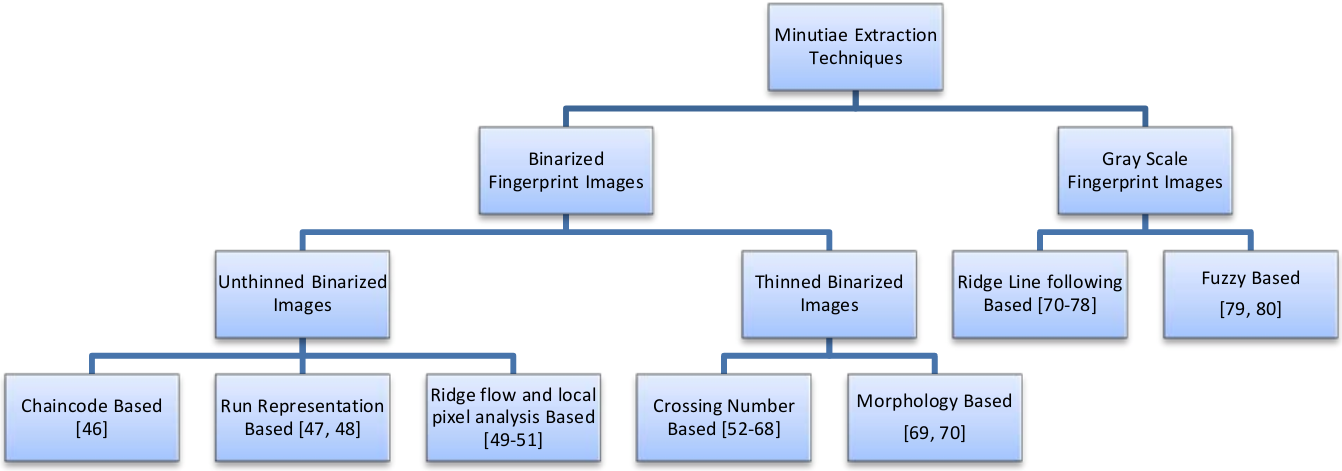
\includegraphics[width=\linewidth]{obrazky-figures/klasifikacia_extrakcie_markantov.png}
    \caption{Rozdelenie rôznych prístupov k extrakcii markantov. Prevzaté z \cite{bansal2011minutiae}.}
    %TODO prerobit tento obrazok z \cite{bansal2011minutiae} na vektorovy (priamo v latexe cez tikz alebo inac).
    \label{obr:diagram_extrakcia_markantov}
  \end{figure}

  \subsection{Binarizované snímky}
  Snímky odtlačkov prstov, ktoré boli prevedené zo snímok s odtieňmi šedej na snímky binárne, resp. výlučne čierno-biele, fungujú na základe skúmania
  lokalizovaného okolia jednotlivých pixelov. Rozoznávajú najmä vzory tvorené kombináciami pixelov v tomto okolí.

  \subsubsection{Run-length kódovanie}
  Jedná sa o spôsob extrakcie markantov na binarizovaných snímkach odtlačkov prstov bez stenčovania papilárnych línií.
  Metóda spočíva v rozpoznaní horizontálnych a vertikálnych behov čiernej v binárnych snímkach. Tieto snímky sú následne reprezentované kaskádou behov,
  pri ktorých sa skontrolujú susediace behy a charakteristické behy. Behy reprezentujú riadky a stĺpce pixelov, ktoré patria papilárnym líniám. Pri určovaní
  behov sa zaznamená pozícia východiskového pixelu a terminálneho pixelu pre daný beh. Následná analýza kaskády behov dokáže určiť jeden z piatich
  prípadov v závislosti od susedných behov:

  \begin{enumerate}
    \item Ne sú prítomné žiadne behy susediace so súčasným behom.
    \item Sú prítomné dva behy susediace so súčasným behom - jeden beh z každej strany.
    \item Je prítomný jeden beh na jednej zo strán súčasného behu.
    \item Sú prítomné dva behy na jednej zo strán súčasného behu.
    \item Je prítomných viac, než dva behy na jednej zo strán súčasného behu.
  \end{enumerate}
  Prípady tri a štyri sú tzv. charakteristické behy, ktoré preukazujú charakteristiky behov pre ukončenia a vidličky v tomto poradí. Druhý prípad je
  tzv. regulárny beh a reprezentuje beh, ktorý je súčasťou priebehu časti papilárnej línie bez markantu. Rozpoznanie charakteristických behov však
  nemusí znamenať, že zodpovedajú ich charakteristickým markantom, pretože iné typy markantov preukazujú charakteristiky ukončenia (napr. bod má dve ukončenia)
  a vidličky (napr. slučka má dve vidličky). Z tohto dôvodu je potrebná následná validácia nájdených charakteristických behov \cite{bansal2011minutiae}.

  \subsubsection*{Extrakcia na základe počtu prechodov}
  Metóda sa aplikuje na binarizované snímky so stenčenými papilárnymi líniami. Je to často využívaná metóda pre jej jednoduchosť výpočtovú rýchlosť.
  Spočíva v počítaní prechodov medzi pixelmi papilárnej línie a pozadím pre každý pixel prislúchajúci papilárnym líniám. Tieto prechody je možné vypočítať
  pomocou masky veľkosti {$3\times{}3$}~(\ref{obr:maska_CN}), ktorá je priložená na jednotlivé pixely papilárnych línií. Na ohľad sú brané
  hodnoty na okrajoch masky (bunky $P_1$ až $P_8$). Zvoleným smerom sa následne prechádzajú páry pixelov prekrývaných okrajovými bunkami masky a vypočíta
  sa kumulatívny rozdiel medzi jednotlivými pármi pomocou vzorca~{\ref{rov:crossing_number}}. Výsledné číslo $C_N$ reprezentuje počet prechodov medzi
  pixelmi pozadia a popredia snímky (angl. crossing number alebo condition number). Z tohto počtu je možné vyvodiť, že ak $C_N = 2$, tak sa jedná o ukončenie,
  a ak $C_N = 6$, tak sa identifikovala vidlička. Všetky ostatné hodnoty $C_N$ sú ignorované \cite{amengual1997minutiae_extraction}.

  \begin{figure}[h]
    \centering
      \begin{tabular}{ | l | c | r | }
        \hline
        $P_6$ & $P_5$ & $P_4$ \\ \hline
        $P_7$ & $P$ & $P_3$ \\ \hline
        $P_8$ & $P_1$ & $P_2$ \\
        \hline
      \end{tabular}
    \caption{Maska veľkosti $3\times{}3$ používaná pri výpočte prechodov medzi pixelmi popredia a pozadia pri metóde CN.}
    \label{obr:maska_CN}
  \end{figure}

  \begin{equation}
    C_N = \sum_{i=1}^{8} | P_{i+1} - P_{i} |, \quad\text{kde } P_9 = P_1
    \label{rov:crossing_number}
  \end{equation}

  \subsection{Snímky v odtieňoch šedej}
  Obyčajne výpočtovo náročnejšie techniky na extrakciu markantov sú techniky zamerané na extrakciu bez binarizácie vstupnej snímky. Výhodou analýzy
  takto neupravenej snímky je, že sa do štruktúr papilárnych línií nedostanú falošné prvky. Pri binarizácii sa totiž môžu nechcene odstrániť časti
  papilárnych vzorov alebo dokonca vytvoriť falošné vzory v~dôsledku nesprávneho prahovania. Pri stenčovaní sa zas môžu vytvárať falošné vedľajšie výbežky
  z~hlavných papilárnych línií. Takáto strata informácií o skutočnom priebehu línií je nežiaduca. Z tohto dôvodu sa skúmali aj možnosti analýzy snímok bez
  takýchto úprav.

  \subsubsection*{Extrakcia markantov sledovaním papilárnych línií}
  Princíp tejto metódy spočíva v sledovaní priebehu papilárnych línií na základe informácií o lokálnej orientácii papilárneho vzoru. Sledovanie sa začne
  zvolením počiatočného bodu $[x_c, y_c]$ a počiatočného smeru $\theta{}_c$. Z tohto bodu sa algoritmus v každom kroku presunie na ďalší bod $[x_t, y_t]$,
  na základe smeru $\theta{}_c$ a veľkosti kroku $\mu$, ktorý udáva počet preskočených pixelov v danom smere. V novom bode sa získajú hodnoty šedej
  naprieč prierezovou sekciou, ktorá je vytvorená kolmo na pôvodný smer $\theta{}_c$ a je dĺžky $2\sigma + 1$. Na základe získaných hodnôt šedej sa
  v rámci sekcie nájde lokálne maximum, pozícia ktorého sa označí ako $[x_n, y_n]$. Tento nový bod sa stáva bodom $[x_c, y_c]$,
  vypočíta sa nový smer $\theta{}_c$ a algoritmus začína novú iteráciu. Algoritmus je znázornený na~{\ref{obr:sledovanie_linii}}.

  \begin{figure}[h]
    \centering
    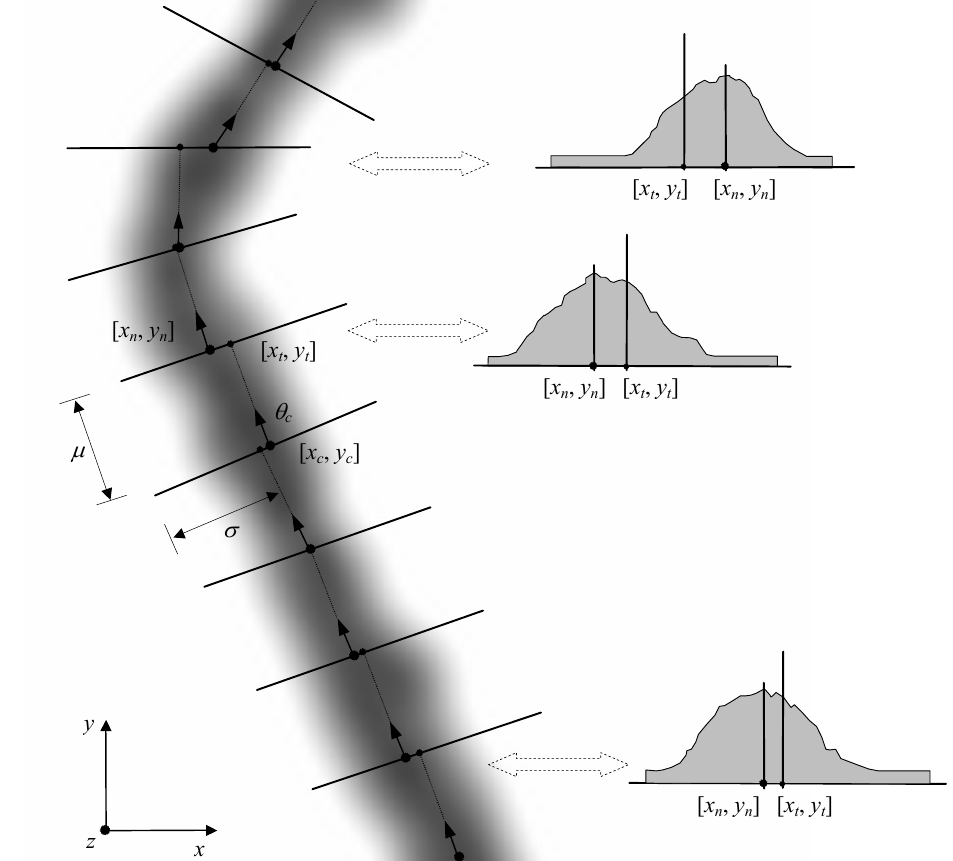
\includegraphics[width=0.65\linewidth]{obrazky-figures/ridge_following-maltoni.png}
    \caption{Znázornenie algoritmu sledovania papilárnych línií. Prevzaté z \cite{Handbook}.}
    \label{obr:sledovanie_linii}
  \end{figure}

  Tento algoritmus je rozširovaný o pomocnú dátovú štruktúru, ktorá zaznamenáva, ktoré časti snímky boli už algoritmom spracované. Toto slúži
  ako prevencia voči viacnásobnému spracovaniu papilárnych línií a zároveň je využívaná pri detekcii markantov. Pomocná snímka $T$ je na začiatku
  extrakcie inicializovaná na prázdnu. Počas sledovania papilárnych línií sa do nej začne ukladať polygonálny obraz skenovaných línií s konštantnou šírkou.
  Na základe porovnávania pomocnej snímky so súčasným krokom sledovacieho algoritmu je možné detegovať pretínanie línií, čo môže znamenať nájdenie markantu
  typu vidlička. Pri ukončených líniách algoritmus deteguje markanty ukončenia \cite{maio1997ridge_following}.

  Existujú variácie vyššie uvedeného algoritmu, ktoré napr. dynamicky upravujú veľkosť kroku $\mu$, alebo ktoré sledujú nielen vrcholy papilárnych línií,
  ale aj susedné údolia \cite{Handbook}.

  \section{Analýza singularít a tried}
  Analýza odtlačkov prstov na prvej úrovni (tzv. hrubá klasifikácia) poskytuje informácie o~vonkajšom vzhľade, resp. priebehu línií odtlačku prsta.
  Na základe informácií tohto priebehu je odtlačky možné klasifikovať do jednej zo šiestich tried (viď. sekcia~{\ref{sec:klasifikacia_odtl}}). Význam
  klasifikácie sa prejavuje najmä pri porovnávaní odtlačkov automatizovanými systémami, a~to v~štádiu hľadania hrubej zhody (zhoda na základe hrubej
  klasifikácie). Tu sa vylučujú z~procesu porovnávania odtlačky, ktorých trieda sa nezhoduje s triedou hľadaného odtlačku, v dôsledku čoho sa značne znižuje
  počet porovnávaní \cite{karu1996classification, Handbook}.

  Značné množstvo prístupov ku klasifikácii využíva prakticky výlučne orientačné pole odtlačku prsta, pretože obecne obsahuje všetky informácie potrebné
  k rozlíšeniu medzi triedami \cite{Handbook}. Avšak prístup na báze pravidiel (viď~{\ref{sec:rule-based}}) využíva aj informácie o singularitách.
  Obecný prístup automatizovanej klasifikácie na báze pravidiel pozostáva z dvoch krokov. Prvým krokom je extrakcia singularít. Historicky jednou
  z najpoužívanejších metód je využitie Poincaré indexu, avšak existujú aj iné prístupy. Druhým krokom je samotný odhad triedy odtlačku.

  \subsection{Detekcia singularít na základe Poincaré indexu}
  Ak máme vektorové pole $G$ a krivku $C$ vsadenú do vektorového poľa $G$, tak Poincaré index $P_{G,C}$ je definovaný ako celková rotácia vektorov $G$ pozdĺž
  krivky $C$ \cite{Handbook}. Táto definícia je ilustrovaná na obrázku~{\ref{obr:poincare_index}}. Metóda detekcie singularít na základe Poincaré indexu vyžaduje
  extrakciu orientácií papilárnych línií (uvedené v sekcii~{\ref{sec:orientacia}}).

  \begin{figure}[h]
    \centering
    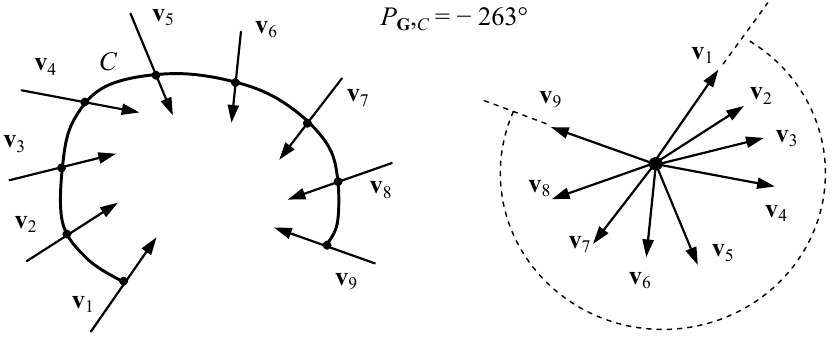
\includegraphics[width=0.65\linewidth]{obrazky-figures/poincare_index.png}
    \caption{Ilustrácia definície Poincaré indexu. Prevzaté z \cite{Handbook}.}
    \label{obr:poincare_index}
  \end{figure}

  Iwasokun a Akinyokun \cite{iwasokun2014singularities} navrhli metódu detekcie jadier a delt na základe Poincaré indexu, ktorý využíva extrahované orientácie
  pomocou metódy navrhnutej v \cite{Hong}. Detekcia singularít funguje nasledovne. V snímke orientácií $O(i,j)$ pre každý pixel $(i,j)$ sa zvolí
  okno veľkosti $3\times{}3$ (znázornené na~{\ref{obr:okno_orientacie}}). V tomto okne sa vypočítajú rozdiely medzi jednotlivými pármi pixelov
  obklopujúcich pixel $O(i,j)$ v smere proti behu hodinových ručičiek~{\ref{eq:poincare_3}}. Toto okno je kruhové, čiže sa počíta aj rozdiel medzi prvým
  a posledným pixelov v okne. Na~základe rozdielov susedných buniek okna sa podľa rovnice~{\ref{eq:poincare_2}} vráti špecifická hodnota $\beta{}_c$.
  Nakoniec sa jednotlivé
  hodnoty $\beta{}_c$ sčítajú. Ak výsledok rovnice~{\ref{eq:poincare_1}} leží v rozsahu \mbox{$<-1;-0,5>$}, tak sa jedná o bod jadra a ak súčet leží
  v rozsahu \mbox{$<0,5;1>$}, jedná sa o~deltu.

  \begin{equation}
    PC(i,j) = \frac{1}{\pi{}} \sum_{c=1}^{8}{\beta{}_c}
    \label{eq:poincare_1}
  \end{equation}
  \begin{equation}
    \beta{}_c = 
    \begin{cases}
      p(c) + \pi{},  & \text{ak } p(c) \leq{} - \frac{\pi{}}{2} \\
      p(c),          & \text{ak } p(c) >  - \frac{\pi{}}{2} \text{ a } p(c) \leq{} \frac{\pi{}}{2} \\
      p(c) - \pi{},  & \text{inak}
    \end{cases}
    \label{eq:poincare_2}
  \end{equation}
  \begin{equation}
    p(c) = O_{c+1} - O_c \quad \text{pričom } O_9 = O_1
    \label{eq:poincare_3}
  \end{equation}

  \begin{figure}[h]
    \centering
      \begin{tabular}{ | l | c | r | }
        \hline
        $O_4$ & $O_5$ & $O_6$ \\ \hline
        $O_3$ & $O(i,j)$ & $O_7$ \\ \hline
        $O_2$ & $O_1$ & $O_8$ \\
        \hline
      \end{tabular}
    \caption{Orientované okno veľkosti $3\times{}3$ okolo pixelu $O(i,j)$ v snímke orientácií.}
    \label{obr:okno_orientacie}
  \end{figure}
  
  Nesprávne detekcie singularít touto metódou je možné odstrániť dvoma spôsobmi:
  \begin{enumerate}
    \item Ak sú delta a jadro od seba vzdialené menej, než 8 pixelov, obe detekcie sú vymazané.
    \item Ak bolo detegovaných viacero (obecne $N$) singularít vo vzdialenosti 8 pixelov od seba, vypočíta sa priemerná poloha singularity zo všetkých
          detegovaných z tejto oblasti.
  \end{enumerate}
  Predísť falošným detekciám singularít je možné vyhladením extrahovaných orientácií lokálnym spriemerovaním ešte pred samotnou detekciu. Toto však môže
  spôsobiť posun bodov singularít smerom k okrajom snímky, avšak existujú metódy pre spätnú korekciu polôh takto posunutých bodov singularít \cite{Handbook}.

  \subsection{Automatizovaná klasifikácia tried odtlačku prsta} \label{sec:auto_klasif}
  Existuje mnoho prístupov ku klasifikácii odtlačkov prsta a obecne ich je možné rozdeliť do jednej z týchto kategórií: \emph{na báze pravidiel},
  \emph{syntaktické}, \emph{štatistické}, \emph{štrukturálne}, \emph{na báze neurónových sietí} a \emph{zložené prístupy}. V tejto sekcii je uvedený
  prístup na báze pravidiel.

  \subsubsection*{Na báze pravidiel} \label{sec:rule-based}
  Často používaným prístupom daktyloskopických expertov ku klasifikácii odtlačkov prstov je aplikácia niekoľkých pravidiel o počte a vzájomnej polohe
  jednotlivých singularít prítomných na odtlačkoch (zobrazené na~{\ref{obr:singularity_v_triedach}}). Tento prístup je možné algoritmizovať a aplikovať
  v automatizovaných systémoch \cite{Handbook}.

  \begin{figure}[h]
    \centering
    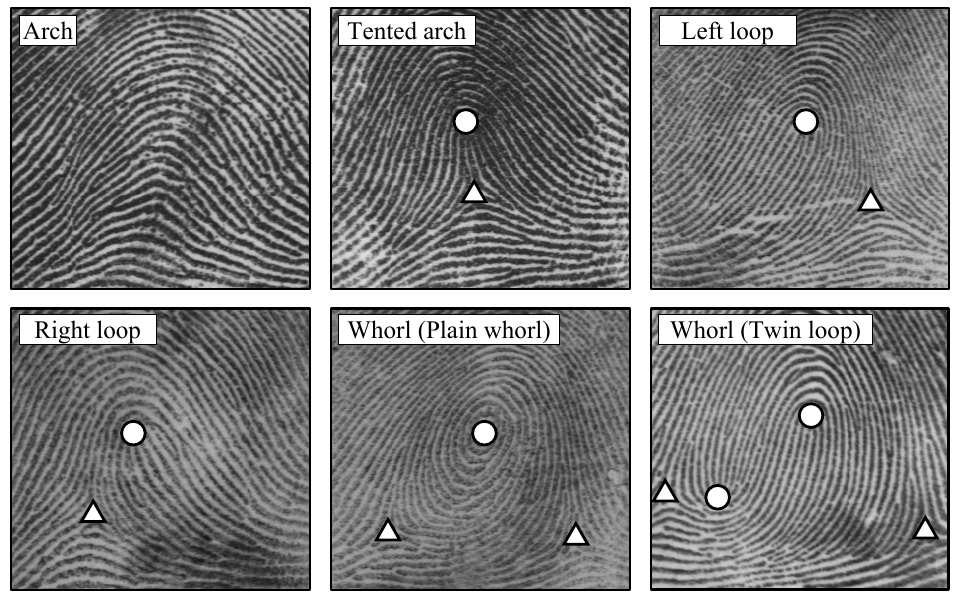
\includegraphics[width=0.85\linewidth]{obrazky-figures/singularity_v_triedach.png}
    \caption{Jednotlivé singularity v rámci rôznych tried odtlačkov prstov. Symboly $\circ{}$ označujú jadrá a $\Delta{}$ označujú delty.
    Prevzaté z \cite{Handbook}.}
    \label{obr:singularity_v_triedach}
  \end{figure}

  Z obrázku~{\ref{obr:singularity_v_triedach}} je možné vyčítať, že triedy odtlačkov prstov sa dajú zaradiť do jednej z~troch kategórií na základe počtu
  singularít nasledovne:
  \begin{enumerate}
    \item v oblúkoch sa nenachádzajú singularity,
    \item v klenutých oblúkoch, ľavých a pravých slučkách je prítomné jedno jadro a jedna delta
    \item a v špirálach a dvojitých slučkách dve jadrá a dve delty (na snímke je pri špirále zobrazené jedno jadro, avšak sa jedná o dve navzájom si čeliace
    prekryté jadrá).
  \end{enumerate}
  V prípade, že odtlačok neobsahuje singularity, je priamo klasifikovaný ako oblúk a odtlačok nevyžaduje bližšiu analýzu. Inak je nutné ďalej analyzovať
  vzájomné pozície nájdených singularít. V prípade, že bol odtlačok zaradený do druhej kategórie, je možné konečnú triedu odhadnúť na základe vzájomnej pozície
  delty a jadra. V prípade, že sklon medzi deltou a~jadrom neprevyšuje istú hranicu, jedná sa o klenutý oblúk. Ak sklon hranicu prevyšuje, je nutné zistiť smer
  odstupu delty spod jadra a zaradiť odtlačok do príslušnej triedy ľavej či pravej slučky - ľavá slučka pri jadre naľavo od delty, pravá slučka v opačnom
  prípade. Rozlíšenie medzi špirálou a dvojitou slučkou zahŕňa prepojenie dvoch jadier priamkou, odmeraním sklonu priamky a priemerného rozdielu orientácií
  pozdĺž tejto priamky \cite{Handbook}.

\chapter{Wavelet Scalar Quantization} \label{kap:wsq}
  Koncom dvadsiateho storočia sa veľmi rýchlo rozrastala zbierka snímok odtlačkov prstov v~FBI, pričom tieto snímky pôvodne neboli komprimované.
  Toto znamenalo stále sa zvyšujúce nároky na úložisko v dátových centrách zabezpečujúcich ukladanie týchto snímok. Digitálne snímky už boli v tejto dobe
  rozšírené, čo znamenalo aj vývoj kompresných formátov pre ukladanie takýchto snímok. Významným formátom bol stratový JPEG (skratka výboru Joint Photographic
  Experts Group), ktorý komprimuje snímky na báze metódy diskrétnej kosínovej transformácie pre jednotlivé bloky snímky veľkosti $8 \times{} 8$. Kompresia touto
  metódou bola uspokojivá z hľadiska bežných užívateľov, avšak spôsob kompresie po diskrétnych blokoch, akým sa kompresia prevádzala, spôsobovalo blokovú
  fragmentáciu. Kvôli takýmto fragmentom sa jemné detaily v snímkach odtlačkov prstov skresľovali vďaka nespojitostiam medzi jednotlivými blokmi,
  čo činilo tento formát neuspokojivým pre ukladanie snímok odtlačkov prstov. Bezstratové kompresné formáty nespôsobovali artefakty, avšak poskytovali
  nedostatočný pomer kompresie ($2:1$ oproti cieľovému pomeru $10,5:1$)~{\cite{Handbook}}.
  
  Z tohto dôvodu bol vyvinutý kompresný algoritmus Wavelet Scalar Quantization (skratkou WSQ, slov.~vlnková skalárna transformácia).
  Jedná sa o algoritmus špecificky vyvinutý na kompresiu snímok odtlačkov prstov, konkrétne tých snímaných s rozlíšením 500 ppi. V~súčasnosti sa
  v kriminalistike naprieč svetom využívajú snímky v odtieňoch šedej s rozlíšením 500 ppi vo formáte WSQ \cite{Libert}.
  Algoritmus WSQ je stratový, čo znamená, že pri kompresii dochádza k istej strate informácií. Bežný pomer kompresie sa pohybuje medzi 10:1 a 15:1,
  pri ktorých spĺňa požiadavky pre maximálnu maximálnu povolenú stratu informácií z originálnej snímky pre účely kriminalistiky \cite{Handbook}.
  Pri zvýšení rozlíšenia snímok odtlačkov prstov na 1000 ppi však formát WSQ nebol na takéto snímky aplikovateľný, kvôli čomu sa pri takýchto rozlíšeniach
  začal využívať formát JPEG 2000 \cite{Libert}.

  Táto kapitola je venovaná základným prvkom formátu WSQ ako je jeho štruktúra a~spôsob kompresie. Jedna sekcia je venovaná aj porovnaní formátov
  WSQ a JPEG 2000.

  \section{Kompresia}
  Algoritmus kompresie a dekompresie využívaný vo formáte WSQ využíva tri hlavné kroky (zobrazené na obrázku~{\ref{obr:WSQ_diagram}}):
  diskrétnu vlnkovú transformáciu (DWT) vstupnej snímky, kvantovanie získaných koeficientov a následné entropické kódovanie kvantovacích indexov~{\cite{Bradley}}.

  \begin{figure}[h]
    \centering
    % //TODO prekreslit toto na PDF vektorovy obrazok
    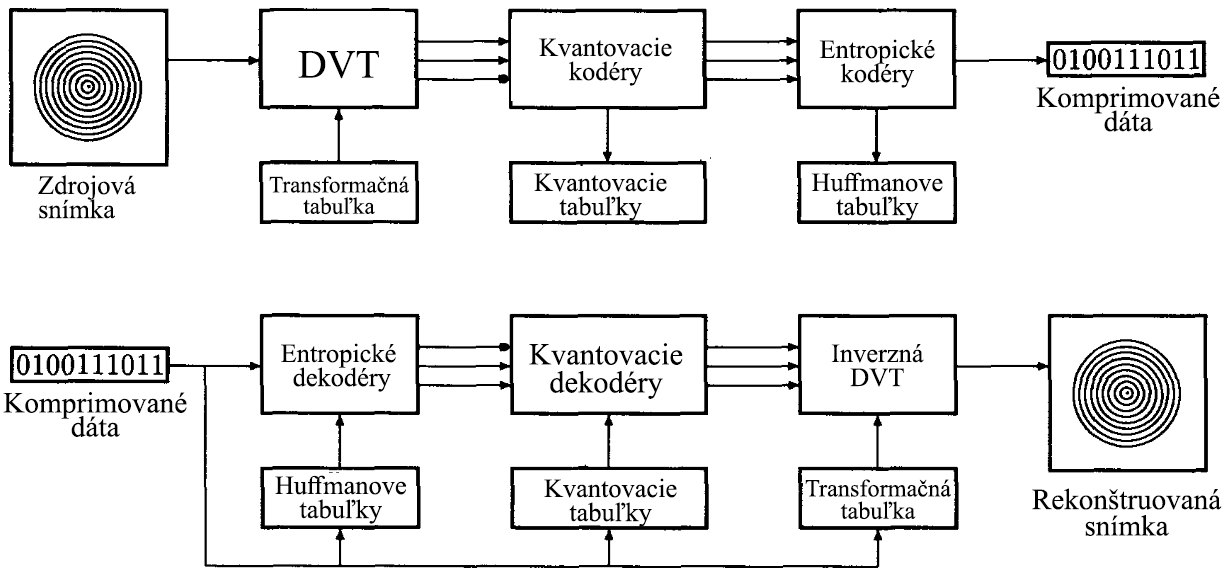
\includegraphics[width=0.8\linewidth]{obrazky-figures/WSQ_encoder_decoder.png}
    \caption{Diagram WSQ kodéra a dekodéra. Prevzaté z \cite{Bradley}.}
    \label{obr:WSQ_diagram}
  \end{figure}
  
  \subsection{Diskrétna vlnková transformácia}
  Prvým krokom v kompresii snímok vo formáte WSQ je diskrétna vlnková transformácia, ktorá prevedie viacúrovňovú dekompozíciu vstupnej snímky na 
  podpásma. Jedna úroveň transformácie je zobrazená na obrázku~{\ref{obr:DWT_uroven}}. Vstupný signál $I$ je rozdelený na podpásma párom filtrov horného
  a dolného priepustu. Tento pár filtrov sa najprv aplikuje pozdĺž riadkov vstupnej snímky (signálu), čo vyprodukuje dva výstupy - jeden výstup reprezentuje
  vstupný signál filtrovaný vysokým priepustom a druhý reprezentuje vstupný signál filtrovaný nízkym priepustom. Tieto dva signály sa následne podvzorkujú
  a sú na ne aplikované rovnaké páry filtrov a následné podvzorkovanie ako v prvom kroku, ale tentoraz po stĺpcoch.

  \begin{figure}[h]
    \centering
    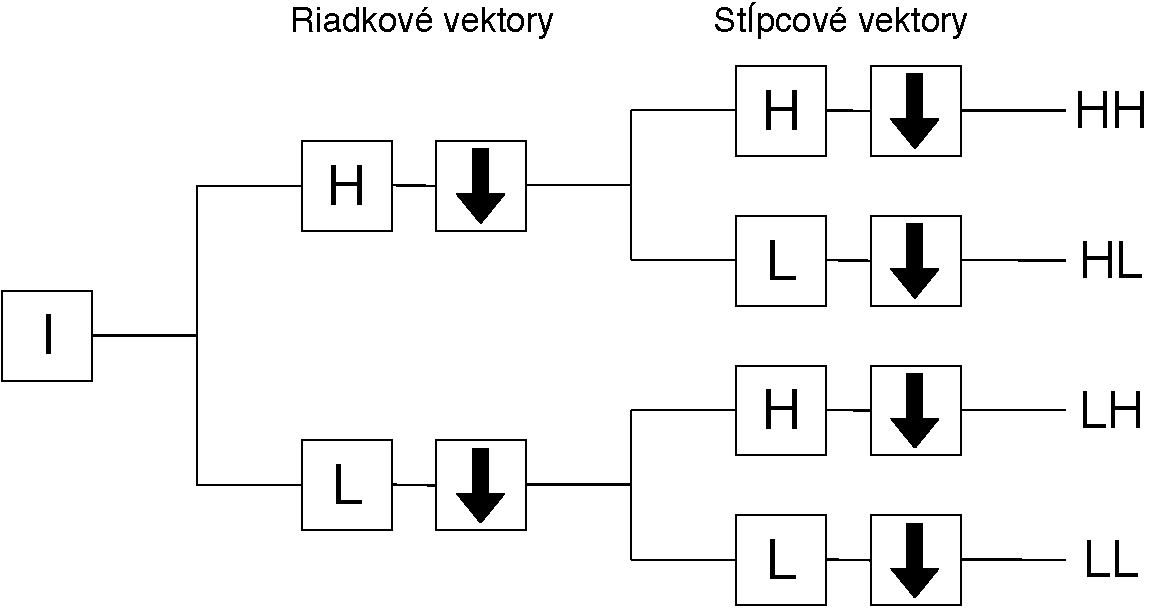
\includegraphics[width=10cm]{obrazky-figures/DWT_level.pdf}
    \caption{Diagram zobrazujúci jednu úroveň rozkladu vstupnej snímky do korešpondujúcich podpásem, kde bloky H predstavujú filtre s horným priepustom,
    bloky L filtre s dolným priepustom, bloky so šípkou nadol značia podvzorkovanie a blok I je vstupný signál. Kombinácie HH, HL, LH a LL reprezentujú
    výstupné signály filtrované vo vyznačenom poradí.}
    \label{obr:DWT_uroven}
  \end{figure}

  Výsledok jednej úrovne takejto transformácie snímky odtlačku prsta je znázornený na obrázku~{\ref{obr:dwt_rozklad_snimky}}. Aproximačná snímka predstavuje
  cestu vstupného signálu (snímky) cez dva filtre nízkeho priepustu, čím sa zachovajú pomalé zmeny vo vstupnom signáli, čiže hrubá štruktúra odtlačku zostáva
  viditeľná. Pre extrakciu vodorovných (a zvislých) detailov bol cez vstupnú snímku aplikovaný najprv jeden druh filtra a následne druhý. Filtre vysokého
  priepustu zachovávajú náhle zmeny priebehu signálu (napr. hrany), čiže v závislosti od smeru, ktorým bol filter cez vstupnú snímku aplikovaný,
  sa extrahujú vodorovné resp. zvislé detaily. Diagonálne detaily sú získané aplikáciou filtra vysokého priepustu v oboch smeroch.

  \begin{figure}[h]
    \centering
    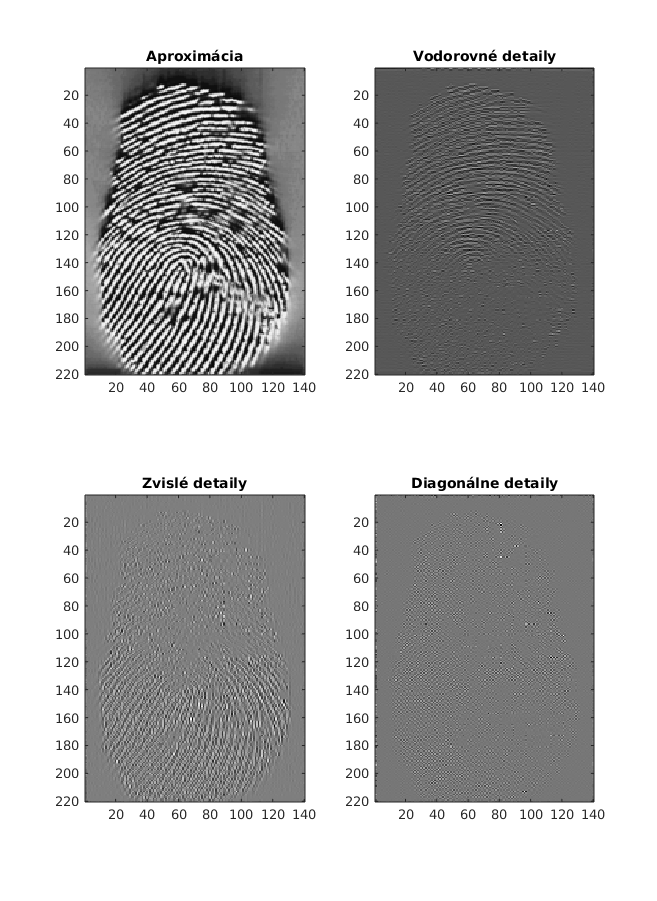
\includegraphics[width=0.5\linewidth]{obrazky-figures/DWT_rozklad_odtlacku.png}
    \caption{Rozklad snímky odtlačku prsta na štyri skupiny koeficientov aplikáciou jednej úrovne diskrétnej vlnkovej transformácie. Vstupná snímka
    z~internej databázy STRaDe.}
    \label{obr:dwt_rozklad_snimky}
  \end{figure}

  Kombináciou typu filtrov a smeru filtrovania sa získavajú štyri skupiny koeficientov transformácie v rôznych smeroch: 
  \begin{itemize}
    \item \emph{LL} produkuje aproximáciu vstupného signálu
    \item \emph{HL} produkuje detaily vo vertikálnom smere
    \item \emph{LH} produkuje detaily v horizontálnom smere
    \item \emph{HH} produkuje detaily v diagonálnom smere.
  \end{itemize}
  Podvzorkovanie faktorom 2 po každom filtrovaní znamená, že výsledná veľkosť dvojrozmerného vektoru jednotlivých koeficientov bude štvornásobne
  menšia, než veľkosť pôvodnej snímky z dôvodu podvzorkovania ako riadkov, tak stĺpcov vstupného signálu.
  Jednotlivé podpásma je možné naďalej kaskádovať cez takúto filtračnú banku, kým sa nedosiahne požadovaná úroveň rozkladu vstupného signálu.

  Formát WSQ aplikuje viacúrovňovú dekompozíciu podpásem naznačenú na obrázku~{\ref{obr:WSQ_DWT_dekompozicia}}, pričom celkovo sa vstupná snímka rozloží
  do 64 podpásem. Obrázok znázorňuje nerovnomerné rozdelenie šírok pásem. Nízke a stredné frekvencie majú alokované úzke pásma, pričom koeficienty vysokých
  frekvencií majú naopak alokované široké pásma. Takéto rozloženie pásem je jednotné pre všetky implementácie kodérov a bolo navrhnuté špecificky pre snímky
  s rozlíšením 500 ppi \cite{brislawn1996compression}.

  \begin{figure}[h]
    \centering
    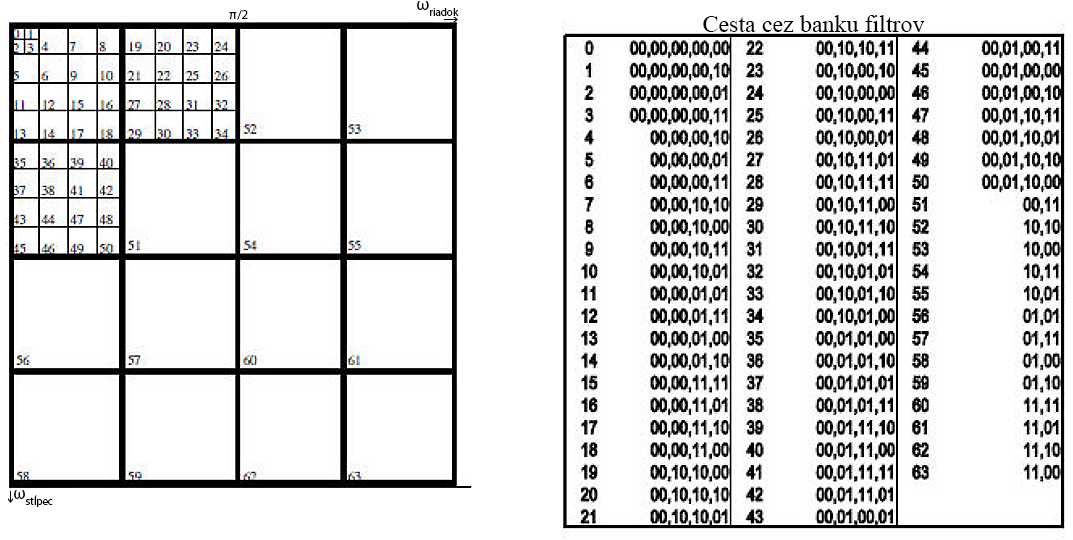
\includegraphics[width=\linewidth]{obrazky-figures/WSQ_DWT_subband_decomposition.png}
    \caption{Dekompozícia podpásem vo formáte WSQ. Zobrazené sú podpásma vo frekvenčnej doméne. V tabuľke napravo je znázornený sled filtrov, ktoré boli
    aplikované na vstupný signál - 1 je filter horného priepustu, 0 je filter dolného priepustu. Prevzaté z \cite{WSQSpecification}.}
    \label{obr:WSQ_DWT_dekompozicia}
  \end{figure}

  \subsection{Kvantovanie}
  Proces kvantovania je spôsob diskretizácie vstupného signálu. V tomto prípade sa jedná o~diskretizáciu koeficientov určených diskrétnou vlnkovou
  transformáciou v predošlom kroku komprimácie. Jednotlivé koeficienty podpásem získaných transformáciou sú uniformne kvantované v rámci každého podpásma,
  čo znamená, že každé podpásmo má vlastný kvantovač. Tento krok zavádza do metódy kompresie zaužívanej vo WSQ stratovosť, pretože hodnoty koeficientov
  sú kvantované z desatinných čísel na celé čísla bez akéhokoľvek zabezpečenia reverzibility tohto procesu.

  \begin{figure}[h]
    \centering
    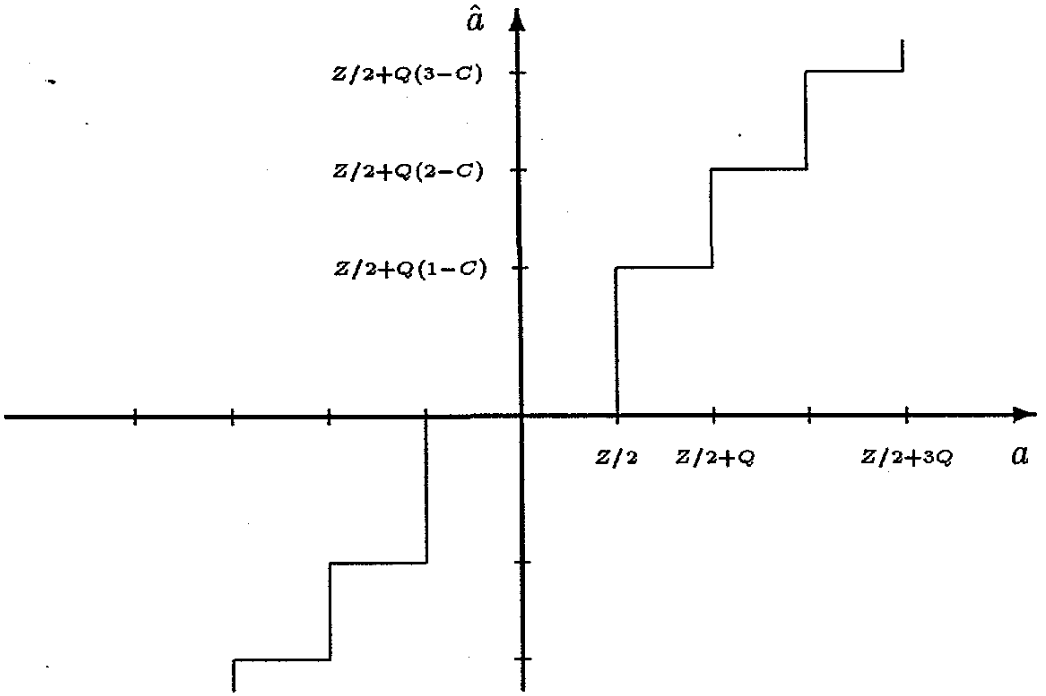
\includegraphics[width=0.6\linewidth]{obrazky-figures/wsq_kvantovacia_charakteristika.png}
    \caption{Kvantovacia charakteristika kvantovača podpásem diskrétnej vlnkovej transformácie. Šírka krokov znázorňuje šírku kvantovacej nádoby.
    Os $a$ reprezentuje kvantovanie a~os $\hat{a}$ reprezentuje reverzné kvantovanie (pri dekompresii). Prevzaté z \cite{brislawn1996compression}.}
    \label{obr:wsq_kvantovacia_charakteristika}
  \end{figure}

  Kvantovanie a jeho reverzná operácia pre dekódovanie komprimovaných snímok sú dané vzťahmi~{\ref{rov:kvantovanie}} a~{\ref{rov:kvantovanie_reverz}}.
  \begin{equation}
    p_k(m,n) =
    \begin{cases}
      \lfloor \frac{a_k(m,n) - Z_k / 2 }{Q_k} \rfloor + 1, & a_k(m,n) > Z_k/2 \\
      0, & -Z_k/2 \leq a_k(m,n) \leq Z_k/2 \\
      \lceil \frac{a_k(m,n) + Z_k / 2 }{Q_k} \rceil - 1, & a_k(m,n) < -Z_k/2 \\
    \end{cases}
    \label{rov:kvantovanie}
  \end{equation}
  \begin{equation}
    \hat{a}_k(m,n) = 
    \begin{cases}
      (p_k(m,n) - C)Q_k + Z_k/2, & p_k(m,n) > 0 \\
      0, & p_k(m,n) = 0 \\
      (p_k(m,n) + C)Q_k - Z_k/2, & p_k(m,n) < 0\\
    \end{cases}
    \label{rov:kvantovanie_reverz}
  \end{equation}
  kde index $k$ označuje $k$-te podpásmo, $a_k(m,n)$ označuje koeficient v danom podpásme, $Z_k$ je šírkou nulovej kvantovacej nádoby,
  $Q_k$ je šírkou nenulovej kvantovacej nádoby a $C$ je centrom kvantovacích nádob pri dekódovaní a zostáva konštantou pre každé podpásmo. {$C$}~je špecifikáciou
  daný ako $C = 0,44$ pre najnovší kodér, pričom $Z_k$ a $Q_k$ sa získa výpočtom rozptylu jednotlivých podpásem. $p_k(m,n)$ označuje kvantovaný koeficient
  zodpovedajúci pôvodnému koeficientu $a_k(m,n)$ a koeficient $\hat{a}_k(m,n)$ je spätne dekódovaný koeficient z~{$p_k(m,n)$}. Funkcie $\lfloor$ $\rfloor$
  a $\lceil$ $\rceil$ definujú zaokrúhlenie na celé číslo smerom nadol a smerom nahor v tomto poradí \cite{WSQSpecification}.

  Všeobecná charakteristika kvantovača pre jedno podpásmo je znázornené na obrázku~{\ref{obr:wsq_kvantovacia_charakteristika}}. Tu je možné vidieť, že šírka
  nultej kvantovacej nádoby $Z$ a šírka zvyšných kvantovacích nádob $Q$ sa líši. Z tohto dôvodu je nutné definovať dve rôzne šírky nádob pre jeden kvantovač.
  Šírky kvantovacích nádob sa definujú špecificky pre danú snímku pri kompresii \cite{brislawn1996compression}.

  \subsection{Entropické kódovanie}
  Ako predpoklad kódovania špecifikácia určuje rozdelenie snímky do minimálne troch blokov, kde prvá hranica je medzi podpásmami 18 a 19 a druhá
  hranica medzi podpásmami 51 a 52. Je to z dôvodu zabezpečenia progresívneho prenosu\footnote{\emph{Progresívny prenos} sa v tomto prípade definuje ako
  metóda prenosu dát takým spôsobom, že nové príchodzie dáta (podpásma vo vyšších frekvenciách) zvyšujú úroveň detailu obsiahnutej v snímke.
  Toto je dosiahnuteľné vďaka charakteristickým vlastnostiam diskrétnej vlnkovej transformácie a spôsobu kódovania dát vo formáte WSQ.}, čo znamená,
  že po sebe nasledujúce bloky pridávajú detaily snímky v progresívne vyšších frekvenciách \cite{WSQSpecification}. Rozdelením podpásem do blokov na týchto
  konkrétnych indexoch zabezpečí možnosť graduálnej rekonštrukcie snímky pridávaním detailov nižšej úrovne dekompozície,
  ako je možné vyčítať zo snímky~{\ref{obr:WSQ_DWT_dekompozicia}}. Rozdelenie do viacerých, než troch blokov je vo WSQ tiež možné s horným limitom obmedzeným
  na 8 blokov \cite{brislawn1996compression}.

  Koeficienty sa v každom podpásme najskôr zoradia v poradí od ľavého horného rohu po pravý dolný roh (teda po diagonálach \uv{cikcakovito})
  a následne sú zakódované pomocou Huffmanovho kódovania. Takéto kódovanie je založené na priradení špeciálnych symbolov pre znaky v reťazcoch na základe
  ich početnosti. Pri WSQ kódovaní koeficientov sa najprv zakódujú nuly na základe dĺžky behu nulových segmentov v zoradenom reťazci kvantovaných koeficientov.
  Tieto kódy sú následne mapované na konečnú množinu symbolov podľa kódovacieho modelu (uvedený v tabuľke~{\ref{tab:kodovaci_model}}). Hodnoty koeficientov,
  ktoré prevyšujú očakávaný kvantovaný rozsah hodnôt $-73$ až $74$ sú označené riadiacim symbolom označujúcim typ (kladná/záporná hodnota) a rozsah (8/16-bit)
  kódovanej hodnoty koeficientu. Týmto nie je nutné stanoviť hraničné hodnoty počas kvantovania, lebo hodnoty nad rozsah sú označené pri
  kódovaní \cite{brislawn1996compression}. Huffmanovo kódovanie zabezpečuje bezstratovú kompresiu koeficientov.

  \begin{table}[ht]
    \centering
    \caption{Kódovací model Huffmanovho kódovania WSQ. Prevzaté z \cite{WSQSpecification}.}
    \begin{tabular}{| c  l |}
      \hline
      \textbf{Symbol} & \textbf{Hodnota} \\
      \hline
      1 & beh núl dĺžky 1 \\
      2 & beh núl dĺžky 2 \\
      \vdots & \vdots \\
      100 & beh núl dĺžky 100 \\
      101 & riadiaci symbol pre kladný 8-bitový koeficient  \\
      102 & riadiaci symbol pre záporný 8-bitový koeficient \\
      103 & riadiaci symbol pre kladný 16-bitový koeficient \\
      104 & riadiaci symbol pre záporný 16-bitový koeficient \\
      105 & riadiaci symbol pre 8-bitovú dĺžku behu núl \\
      106 & riadiaci symbol pre 16-bitovú dĺžku behu núl \\
      107 & hodnota $-73$ indexu kvantovacej nádoby \\
      108 & hodnota $-72$ indexu kvantovacej nádoby \\
      \vdots & \vdots \\
      180 & nevyužité - použije sa symbol 1 \\
      \vdots & \vdots \\
      253 & hodnota $73$ indexu kvantovacej nádoby \\
      254 & hodnota $74$ indexu kvantovacej nádoby \\
      \hline
    \end{tabular}
    \label{tab:kodovaci_model}
  \end{table}

  \section{Štruktúra súboru} \label{sec:struktura}
  Súbory tvorené snímkami komprimovanými algoritmom WSQ majú definovanú štruktúru. Tieto súbory v sebe nesú informácie potrebné pre úspešnú
  dekompresiu snímok, čo znamená, že obsahujú transformačnú tabuľku, kvantovaciu tabuľku a Huffmanovu tabuľku vrátane ich metadát.
  Samotná štruktúra súboru vo formáte WSQ je podobná tej vo formáte JPEG. Jednotlivé časti súboru sú oddelené dvojbytovými značkami,
  zobrazenými v tabuľke~{\ref{tab:znacky_WSQ_suboru}}, reprezentujúce začiatky segmentov v súbore. Niektoré segmenty obsahujú dodatočné parametre,
  ktoré popisujú dĺžku, vnútornú štruktúru a hodnoty daných segmentov.

  \begin{table}[ht]
    \centering
    \caption{Dvojbytové značky vo WSQ súboroch. Prevzaté z \cite{WSQSpecification}.}
    \begin{tabular}{ |l c l| }
      \hline
      Značka & Skratka označenia & Vysvetlivka \\
      \hline
      FFA0h       & SOI  & Začiatok snímky \\
      FFA1h       & EOI  & Koniec snímky \\
      FFA2h       & SOF  & Začiatok rámca \\
      FFA3h       & SOB  & Začiatok bloku \\
      FFA4h       & DTT  & Definícia transformačnej tabuľky \\
      FFA5h       & DQT  & Definícia kvantovacej tabuľky \\
      FFA6h       & DHT  & Definícia Huffman tabuľky (tabuliek) \\
      FFA7h       & DRI  & Definícia reštart intervalu \\
      FFA8h       & COM  & Komentár \\
      FFB0h-FFB7h & RSTm & Reštartuj s modulo 8 počet m (kde m=0-7) \\
      \hline
    \end{tabular}
    \label{tab:znacky_WSQ_suboru}
  \end{table}

  Samotný súbor je možné rozdeliť na tri hlavné úrovne vnorenia. \\
  \emph{Na prvej úrovni} sa nachádzajú značky \textbf{SOI} a \textbf{EOI}, ktoré definujú začiatok a koniec prenosu výmenného formátu
  (angl. interchange format) komprimovanej snímky. Tieto značky nemajú so sebou asociované žiadne dáta a slúžia výlučne ako označenia. \\
  \emph{Na druhej úrovni} sa nachádza tzv. rámec, ktorého začiatok sa označuje značkou \textbf{SOF}. Rámce v sebe nesú metadáta o obsahu daného rámca ako
  napríklad dĺžku rámca, počet riadkov a stĺpcov zdrojovej snímky\footnote{Tieto hodnoty sú 16-bitové, čo znamená, že maximálna veľkosť komprimovanej snímky
  je $65536 \times 65536$. Bežná veľkosť snímok WSQ sa však pohybuje medzi $780\times 780$ až $1625 \times 975$ pri 520 ppi v závislosti od veľkosti
  zaznamenávaných častí skenovaných daktyloskopických kariet \cite{hopper_wsq_format}.}, umiestnenia hodnôt transformačných parametrov, identifikáciu softvéru,
  ktorý kódoval túto snímku apod. Medzi značkami \textbf{SOI} a \textbf{EOI} sa musí nachádzať výlučne jeden rámec. \\
  \emph{Na tretej úrovni}, v rámci rámca, sú bloky nachádzajúce sa po hlavičke rámca (nie je to pravidlo, upresnenie nižšie) a sú označované značkou
  \textbf{SOB}. Tieto bloky obsahujú hlavičky s informáciou o dĺžke hlavičky bloku a číslo (selektor) Huffmanovej tabuľky pre dekódovanie dát v bloku.
  Bloky obsahujú segmenty entropicky kódovaných dát kvantovaných koeficientov. Každé podpásmo má vlastný blok. Na tejto úrovni sa nachádzajú aj reštart
  značky (\textbf{RSTm}), ak sú povolené. Ak reštart značky v súbore povolené nie sú, počet segmentov kódovaných dát v bloku nesmie byť vyšší, než 1
  a žiadne reštart značky nesmú byť v bloku prítomné.

  Segmenty s údajmi o tabuľkách (transformačné, kvantovacie a Huffmanove) a komentáre nemajú definované \emph{presné} umiestnenie, avšak je obmedzené,
  na ktoré miesta v súbore je možné tieto segmenty vkladať. Tieto umiestnenia sú dve, a to medzi značkou \textbf{SOI} a~{\textbf{SOF}}, prípadne pred ktorýmkoľvek
  blokom. Definičné segmenty tabuliek obsahujú informácie o~dĺžkach týchto definičných segmentov a informácie špecifické pre jednotlivé tabuľky pre správne
  dekódovanie (Huffman tabuľka), spätné kvantovanie (kvantovacia tabuľka) a~spätnú kompozíciu (transformačná tabuľka) komprimovanej
  snímky \cite{WSQSpecification,brislawn1996compression}.

  \section{Porovnanie WSQ s JPEG 2000}
  Formát JPEG 2000 (tiež známy ako JPEG2K) je medzinárodný ISO (názov medzinárodnej organizácie pre normalizáciu) štandard pre kompresiu snímok.
  Jedná sa o tzv. decoder-only štandard, čo znamená, že nekladie obmedzenia
  na pomer kompresie (môže sa jednať aj o bezstratovú kompresiu), ale umožňuje extrémne flexibilnú dekompresiu. Medzi vlastnosti tejto flexibility patrí
  schopnosť dekódovania snímky do ľubovolnej úrovne kvality a~rozlíšenia a dokonca podpora rôznej kvality dekódovania rôznych častí snímky. Štandard podporuje
  snímky veľkosti niekoľkých tisícov terapixelov s~hĺbkou detailu až 38 bitov na vzorku\footnote{Informácie z webovej stránky JPEG pre štandard JPEG 2000
  \url{https://jpeg.org/jpeg2000/} zo dňa 11.7.2020}. Kompresná technológia tohto formátu je, podobne ako u WSQ, založená na
  vlnkovej transformácií, čo znamená, že pri kompresii sa netvoria štvorcové fragmenty ako u jeho predchodcu, formátu JPEG. Tieto vlastnosti spravili z tohto
  štandardu kandidáta FBI na formát pre snímky odtlačkov prstov vyššej kvality. Štandard JPEG 2000 bol zavádzaný po dvoch častiach, kde prvá časť obsahovala
  špecifikácie, ktorých aplikácia bola požadovaná od každej implementácie tohto štandardu. Druhá časť rozvoľňovala reštriktívnu politiku prvej časti popísaním
  voliteľných funkcionalít, ktorými je možné rozšíriť dekodér špecifikovaní v~prvej časti \cite{lepley2001jpeg,Libert}.

  Práca \cite{lepley2001jpeg} sa zamerala na porovnanie interoperability medzi vtedy novým štandardom JPEG 2000 a WSQ, a to špecificky, či bude možné
  transkódovať\footnote{Transkódovanie v tomto prípade myslené ako schopnosť prevedenia komprimovaných dát z formátu WSQ do formátu JPEG 2000 bez nutnosti
  spätnej transformácie do pôvodnej snímky a opätovnej dekompozície pre zakódovanie štandardom JPEG 2000.} súbory WSQ do JPEG~2000. Zistenia potvrdili,
  že transkódovanie je možné vďaka druhej časti špecifikácie bez vizuálnej straty. V prípade transkódovania pomocou časti 1 boli zistené väčšie straty
  na kvalite obrazu.

  Výskum rozdielov kompresných algoritmov medzi WSQ a JPEG 2000 bol vykonaný v~práci \cite{Libert}. Tento výskum bol zameraný na porovnanie straty detailu
  v komprimovaných snímkach algoritmami týchto dvoch formátov. Pre analýzu rozdielov medzi týmito algoritmami bola využitá implementácia OpenJPEG,
  čo je open-source JPEG 2000 kodek. Štúdia sa zamerala na tri primárne prípady kompresie pôvodne nekomprimovaných snímok:
  \begin{enumerate}
    \item Kompresia jedným kompresným cyklom pri oboch algoritmoch a vzájomné porovnanie vrcholového pomeru signálu k šumu, ako aj rozdiely spektrálneho
          výkonu oproti pôvodnej snímke pri 500 ppi snímkach s kompresným pomerom 15:1.
    \item Kompresia dvoma kompresnými cyklami rovnakého kodeku z dôvodu študovania progresívneho dopadu straty detailov pri opakovanej kompresii.
    \item Kompresia dvoma kompresnými cyklami opačných kodekov z dôvodu študovania dopadu straty detailov komprimáciou jedným kodekom a opätovnou komprimáciou
          druhým kodekom.
  \end{enumerate}
  Výsledky kompresie JPEG 2000 poukazujú na menšie zachovanie detailov v strednej frekvenčnej šírke snímky, v ktorej sa bežne nachádzajú detaily odtlačkov
  prstov využívaných pre identifikáciu. Zistenia štúdie preukazujú veľmi vysokú stabilitu zachovania kvality snímky pri kodeku JPEG 2000 za dvojnásobnej
  komprimácie. Pri dvojnásobnej kompresii opačnými kodekmi výsledky poukazujú na značné zníženie kvality snímky \cite{Libert}. V roku 2014 bola vydaná
  príručka pre kompresiu odtlačkov prsta snímaných s rozlíšením 1000 ppi \cite{orandi2014guidance}. Príručku vydal NIST (National Institute of Standards
  and Technology) v spolupráci s FBI.

\chapter{Návrh a implementácia aplikácie} \label{kap:navrh_appky}
  V tejto kapitole je uvedený popis aplikácie zameranej na demonštráciu prístupov k analýze snímkov odtlačkov prstov. Sú tu uvedené využité algoritmy
  predspracovania a spracovania vstupnej snímky, ako aj algoritmy analýzy snímok odtlačkov prstov spolu s popisom ich implementácie. Nakoniec sú uvedené
  problémy implementácie a diskusia o možných vylepšeniach.

  \section{Návrh}
  Aplikácia je rozdelená na dve primárne časti: grafické rozhranie a väzby funkcií naň. Grafické rozhranie poskytuje užívateľovi možnosti aplikácie
  rôznych krokov predspracovania a~analýzy snímok odtlačkov prstov. Väzby funkcií poskytujú rozhranie medzi grafickým rozhraním a algoritmami spracovania
  snímok. Vlastne sa jedná o frontend-backend návrh, zobrazený na obrázku~{\ref{obr:sucasti_app}}.

  \begin{figure}[h]
    \centering
    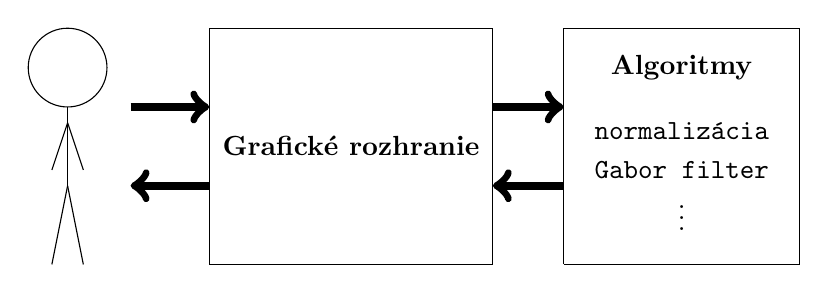
\begin{tikzpicture}
      % uzivatel
      \draw (0.2,2.5) circle (0.5);
      \draw (0.2,2) -- (0.2,1);
      \draw (0.2,1.8) -- (0,1.2);
      \draw (0.2,1.8) -- (0.4,1.2);
      \draw (0.2,1) -- (0,0);
      \draw (0.2,1) -- (0.4,0);
      % GUI stvorec
      \draw (2,0) -- (5.6,0) -- (5.6,3) -- (2,3) -- (2,0);
      \draw (3.8,1.5) node {\textbf{Grafické rozhranie}};
      % algortimy stvorec
      \draw (6.5,0) -- (9.5,0) -- (9.5,3) -- (6.5,3) -- (6.5,0);
      \draw (8,2.5) node {\textbf{Algoritmy}};
      \draw (8,1.7) node {\texttt{normalizácia}};
      \draw (8,1.2) node {\texttt{Gabor filter}};
      \draw (8,0.7) node {\vdots{}};
      % sipky medzi nimi
      \draw[-to, line width=3pt] (1,2) -- (2,2);
      \draw[to-, line width=3pt] (1,1) -- (2,1);
      \draw[-to, line width=3pt] (5.6,2) -- (6.5,2);
      \draw[to-, line width=3pt] (5.6,1) -- (6.5,1);
    \end{tikzpicture}
    \caption{Zobrazenie rozloženia súčastí aplikácie.}
    \label{obr:sucasti_app}
  \end{figure}

  Grafické rozhranie je individuálnym modulom, ktorý volá na základe vstupov užívateľa funkcie jednotlivých algoritmov. Grafické rozhranie sa stará
  o prezentáciu dát - teda o~interpretáciu spracovaných dát, pričom jednotlivé moduly algoritmov spracúvajú vstupné dáta snímky a vracajú ich v rovnakých
  dimenzionálnych rozmeroch ako vstupné. Týmto sa aplikácia činí sčasti modulárnou, pretože algoritmy nie sú prakticky\footnote{Okrem signatúry funkcie
  algoritmu.} nijak viazané na grafické rozhranie.

  Cieľom aplikácie je poskytnúť jednoduchý prehľad o zaužívaných metódach predspracovania a analýzy snímok odtlačkov prstov. Dôraz bol teda kladený na
  čo najjednoduchšie grafické prevedenie bez rušivých elementov. Všetky možnosti spracovania by mali byť uvedené v jednom paneli s vhodným rozdelením podľa
  účelu jednotlivých operácií. Pre často vykonávané úkony ako načítanie novej snímky, export spracovanej snímky a priblíženie je vhodné priradiť
  klávesové skratky pre zjednodušenie ovládania.

  \section{Využité technológie}
  Aplikácia je napísaná v jazyku Python verzie 3.5.3. Na rozhodnutie využiť tento jazyk mal najväčší dopad jeho prenositeľnosť a vysoká podpora nástrojov,
  obzvlášť v smere dátovej manipulácie. Primárnymi modulmi aplikácie sú PyQt5 pre grafické rozhranie a~{\texttt{numpy}} a \texttt{scipy} pre dátovú manipuláciu.
  Všetky požadované moduly sú uvedené v exportovanom súbore \texttt{requirements.txt} v priečinku so zdrojovými súbormi. Tento súbor slúži aj ako
  podporný súbor pri inštalovaní požadovaných modulov (spôsob inštalácie aplikácie je uvedený v prílohe~{\ref{sec:instalacia}}).

  \begin{itemize}
    \item Grafické rozhranie je postavené na aplikačnom rámci PyQt5. Tento rámec je jedným z dvoch rozšírených Python väzieb\footnote{Týmito rozšírenými
          väzbami sú PyQt a PySide.}
          na multiplatformový, voľne dostupný GUI toolkit Qt.
    \item Pre importovanie a exportovanie snímok sa využila knižnica Pillow (fork knižnice PIL). Jedná sa o knižnicu pre spracovanie obrázkov,
          ktorá poskytuje mnoho funkcionalít, avšak v rámci tejto aplikácie sa primárne využíva iba pre načítanie snímok odtlačkov prstov a ukladanie
          ich spracovaných variánt.
    \item Samotné úpravy snímok a algoritmy pre ich spracovanie využívajú knižnice \texttt{numpy}, prípadne \texttt{scipy}. Tieto knižnice sú vhodné pre
          spracovanie viacrozmerných reprezentácií snímok a pre aplikáciu operácií nad nimi.
  \end{itemize}

  \section{Grafické rozhranie}
  Grafické rozhranie pozostáva z ovládacieho panelu, pomocou ktorého je možné vykonávať operácie nad snímkami a z ukážky súčasne
  spracovávaného odtlačku prsta (znázornené na~{\ref{obr:app}}). Ukážka reflektuje úkony vykonávané na snímke pomocou ovládacieho panelu. Ovládací panel
  obsahuje výber jednotlivých filtrov, transformácii a iných úkonov.
  \begin{figure}[h]
    \centering
    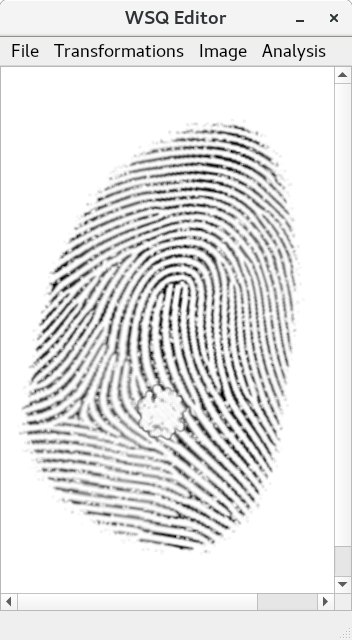
\includegraphics[width=0.4\linewidth]{obrazky-figures/app.png}
    \caption{Vzhľad aplikácie s načítanou snímkou syntetického odtlačku prsta z internej databázy STRaDe.}
    \label{obr:app}
  \end{figure}
  Základom aplikácie sú triedy \texttt{MainWindow} definujúca logiku aplikácie a \texttt{Ui\_MainWindow} definujúca vzhľad aplikácie.

  \subsection{\texttt{MainWindow}}
  Hlavná trieda grafického rozhrania, ktorá riadi beh a komunikáciu aplikácie s užívateľom pomocou definovaných metód viazaných na rôzne akcie.
  Zabezpečuje správne prepojenie týchto akcií s algoritmami a zobrazovanie, či už originálnych alebo spracovaných, snímok.

  Metóda \texttt{open} zabezpečuje načítanie vstupnej snímky a jej následné zobrazenie. Pri požiadavke užívateľa o otvorenie novej snímky zobrazí
  dialógové okno s prehliadačom súborov s možným filtrovaním obrazových súborov. Metóda zvolený súbor skontroluje, či sa jedná o podporovaný formát.
  V prípade, že áno, snímku načíta a zobrazí.

  Metóda \texttt{showImage} sa stará o správnu interpretáciu snímky, ktorú je potrebné zobraziť. Vzhľadom na to, že snímky sa interne ukladajú ako
  dvojrozmerné polia triedy \texttt{ndarray} knižnice \texttt{numpy}, je potrebné vykonať konverziu do triedy \texttt{QImage} knižnice PyQt. Okrem tejto
  konverzie zabezpečuje aj interpretáciu neštandardných dátových typov ako sú binárne snímky alebo float snímky a ich konverziu do dátových typov a rozsahov
  hodnôt, ktoré je \texttt{QImage} schopné interpretovať ako snímku.

  Táto trieda implementuje aj metódy prepájajúce externé algoritmy spracovania a analýzy snímok s grafickým rozhraním, a to spôsobom, že sa jednotlivé
  vstupné akcie vykonateľné užívateľom naviažu na tieto metódy. Väzbu zabezpečuje trieda \texttt{QAction}. Definícia akcie zahŕňa aj voliteľnú  voľbu
  klávesovej skratky. PyQt zabezpečuje naslúchanie klávesovým skratkám a pri ich stlačení zavolá definovanú callback metódu príslušnej akcie.

  \subsection{\texttt{Ui\_MainWindow}}
  Táto trieda bola generovaná automaticky z exportovaného \texttt{.ui} súboru vytvoreného aplikáciou Qt Creator. Jedná sa o aplikáciu pre navrhovanie
  grafických rozhraní pre využitie v~súbehu s GUI toolkitom Qt. Pomocou tohto nástroja bolo navrhnuté a následne exportované GUI vytváranej aplikácie. Súbory
  \texttt{.ui} sú vlastne XML reprezentáciou návrhu grafického rozhrania a je možné ich preložiť do PyQt zápisu. Trieda \texttt{Ui\_MainWindow} je výsledkom
  tohto prekladu. Dedením tejto triedy triedou \texttt{MainWindow} je zabezpečené oddelenie definície vzhľadu aplikácie a jej logiky, čo prispieva k
  prehľadnejšiemu kódu.

  \section{Algoritmy}
  V tejto sekcii sú popísané jednotlivé využité algoritmy a ich implementácia v aplikácii.
  Základnými úpravami, ktoré sa vykonávajú pred každým iným druhom spracovania sú normalizácia a filtrovanie Butterworth filtrom.
  Normalizácia snímky sa vykonáva pomocou funkcie \texttt{normalizeMeanVariance}, ktorá implementuje metódu
  popísanú v sekcii~{\ref{sec:normalizacia}}, čo znamená, že normalizuje pomocou úpravy strednej hodnoty a rozptylu hodnôt pixelov v~snímke. Tento úkon je
  vykonávaný pred každým iným druhom spracovania.\\
  Butterworth filtrovanie prebieha vo frekvenčnej doméne snímky. Frekvenčná reprezentácia snímky je získaná dvojrozmernou rýchlou Fourierovou transformáciou.
  Pre danú snímku je vytvorený filter dolného priepustu, ktorý sa aplikuje vo frekvenčnej doméne na danú snímku. Nakoniec sa filtrované spektrum inverznou
  transformáciou prevedie do pôvodnej, priestorovej, reprezentácie. Týmto sa odstránia zo snímky vysokofrekvenčné fragmenty ako napríklad textúra papiera
  pri skenovaných snímkoch odtlačkov prstov. Toto filtrovanie sa vykonáva vo funkcii \texttt{butterworth}. Originály zobrazovaných snímok odtlačkov prstov
  pochádzajú z internej databázy STRaDe.

  \subsection{Orientácia papilárnych línii}
  Snímka orientácií je získaná pomocou funkcie \texttt{ridgeOrient}. Gradient v smeroch $x$ a $y$ sa získa konvolúciou snímky Sobel filtrami v oboch smeroch.
  Z gradientov sa prepočítajú vektorové polia v oboch smeroch a z nich sa následne získa orientačná snímka s orientáciami v radiánoch.
  Na obrázku~{\ref{obr:orientacie}} je zobrazená snímka po filtrovaní Sobel filtrom a jej konečná podoba po interpretácii orientácií pre zobrazenie.

  \begin{figure}[h]
    \centering
    \begin{subfigure}[b]{0.3\linewidth}
      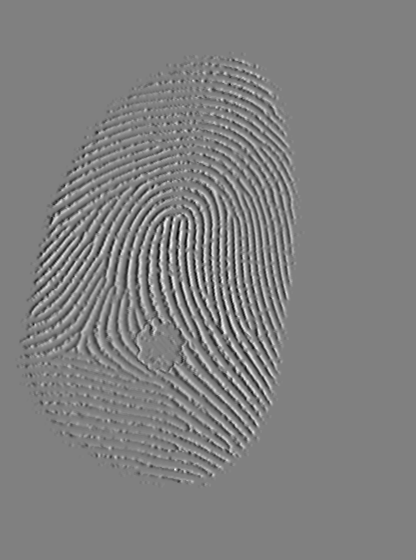
\includegraphics[width=\linewidth]{obrazky-figures/dX.png}
      \caption{snímka detailov v smere $x$}
    \end{subfigure}
    \hfill
    \begin{subfigure}[b]{0.3\linewidth}
      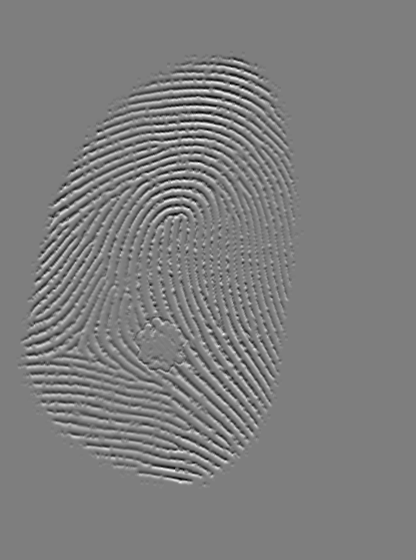
\includegraphics[width=\linewidth]{obrazky-figures/dY.png}
      \caption{snímka detailov v smere $y$}
    \end{subfigure}
    \hfill
    \begin{subfigure}[b]{0.3\linewidth}
      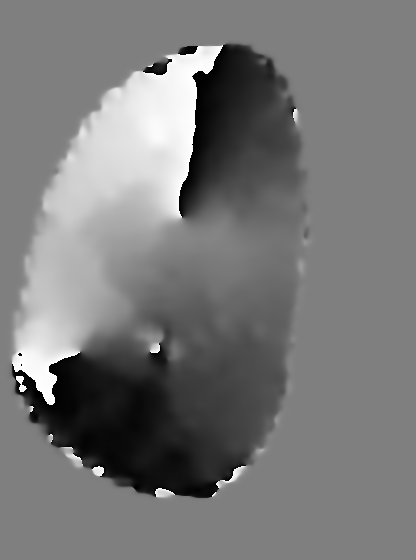
\includegraphics[width=\linewidth]{obrazky-figures/orientim.png}
      \caption{snímka orientácií}
    \end{subfigure}
    \caption{Vizualizácia detailov v dvoch smeroch snímky a konečná snímka orientácií.}
    \label{obr:orientacie}
  \end{figure}

  \subsection{Frekvencia papilárnych línií}
  Algoritmus je riadený funkciou \texttt{ridgeFreq}. V tejto funkcii sa iteratívne prechádza blokmi snímky, ktoré sú následne natočené podľa priemernej
  orientácie v tomto bloku tak, aby papilárne línie boli kolmé na os $x$. V takto natočenom bloku sú následne spriemerované hodnoty po stĺpcoch
  a extrahovaná $x$-signatúra línií. Z tejto signatúry sa vypočíta priemerná frekvencia v danom bloku a vytvorí sa nová snímka frekvencií. Táto snímka
  obsahuje lokálne frekvencie papilárnych línií po diskrétnych blokoch, pričom susedné bloky môžu mať značne odlišné hodnoty. Takéto správanie zdravé papilárne
  línie nepreukazujú a preto je na túto snímku aplikované Gaussovské rozostrenie (priemerovanie), čím sa \uv{spomalý} prechod medzi jednotlivými blokmi.
  Rozdiel medzi pôvodnou frekvenčnou snímkou a rozostrenou verziou je možné vidieť na obrázku~{\ref{obr:frekvencie}}. Význam tohto rozostrenia je zreteľný pri
  kroku Gabor filtrovania, ktoré je popísané v sekcii \ref{sec:gabor_algo}.

  \begin{figure}[h]
    \centering
    \begin{subfigure}[b]{0.3\linewidth}
      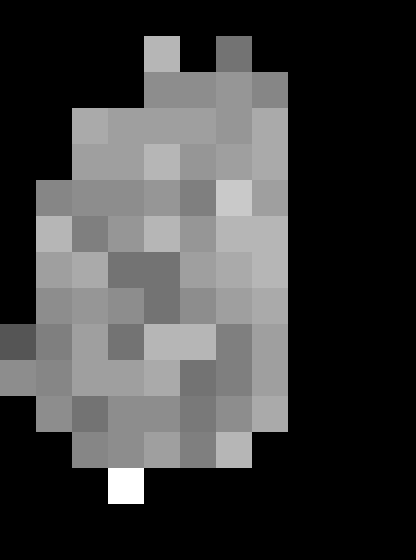
\includegraphics[width=\linewidth]{obrazky-figures/freqim.png}
      \caption{pôvodná frekvenčná snímka}
    \end{subfigure}
    \hspace{0.05\linewidth}
    \begin{subfigure}[b]{0.3\linewidth}
      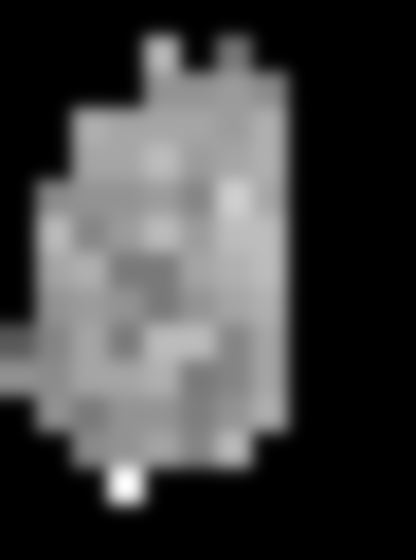
\includegraphics[width=\linewidth]{obrazky-figures/freqim_blur.png}
      \caption{rozostrená frekvenčná snímka}
    \end{subfigure}
    \caption{Snímky frekvencií.}
    \label{obr:frekvencie}
  \end{figure}

  \subsection{Gabor filtrovanie} \label{sec:gabor_algo}
  Funkcia \texttt{gaborFilter} prijíma štyri hlavné parametre, a to pôvodnú snímku, snímku orientácií, frekvencií a masku oblasti záujmu. Pre každý pixel
  snímky, ktorý sa nachádza v oblasti záujmu je následne vygenerovaný vlastný kernel Gabor filtra na základe príslušných dát o~frekvencii a orientácii
  snímky v tom danom pixeli. Tento kernel sa konvolúciou aplikuje na súčasný pixel a hodnota sa zapíše do nového dvojrozmerného poľa rovnakej veľkosti ako
  vstupná snímka. Po prejdení každého požadovaného pixelu sú hodnoty získané filtráciou prahované pre získanie binárnej snímky.

  Na obrázku~{\ref{obr:gabor}}
  je možné pozorovať filtrovanú snímku pred a po binarizácii. Štvorcové fragmenty na prvých dvoch zobrazených snímkach sú tvorené tým, že snímka frekvencií je
  diskrétna po blokoch, čím sa niekedy tvoria značné skoky vo frekvenciách parametrov filtra susedných pixelov. Tretia snímka bola získaná filtrovaním na základe
  priemerovanej frekvenčnej snímky zbavenej náhlych prechodov medzi susednými blokmi frekvencií. Vďaka tomuto priemerovaniu bolo predídené výrazným štvorcovým
  fragmentom, čo podporilo kvalitnejšiu binarizáciu.

  Kvôli blokovým fragmentom je totiž obtiažne prahovať snímku, a to nie len pomocou globálneho prahu. Snímky \ref{obr:gabor_binar} a
  \ref{obr:gabor_binar_freq_blur} boli obe binarizované adaptívne, pričom je zjavné, že výsledok druhej z týchto snímok je značne vyššej kvality bez výrazných
  fragmentov. Samotná binarizácia je vykonávaná po blokoch, v rámci ktorých sa vypočíta optimálny prah. Na základe tohto prahu sa v každom bloku prahujú hodnoty,
  čím sa získa binárna snímka. Výhodou takejto binarizácie oproti prevedeniu s globálnym prahom je, že berie na ohľad kontext okolných pixelov práve
  binarizovaného pixelu, vďaka čomu sa získa kvalitnejšie binarizovaná snímka.

  \begin{figure}[h]
    \centering
    \begin{subfigure}[b]{0.3\linewidth}
      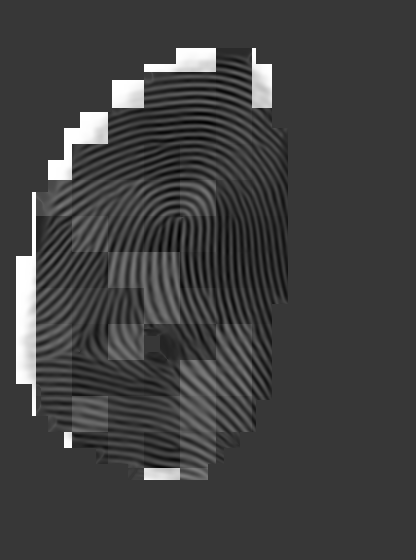
\includegraphics[width=\linewidth]{obrazky-figures/gabor_filtered.png}
      \caption{nebinarizovaná}
    \end{subfigure}
    \hfill
    \begin{subfigure}[b]{0.3\linewidth}
      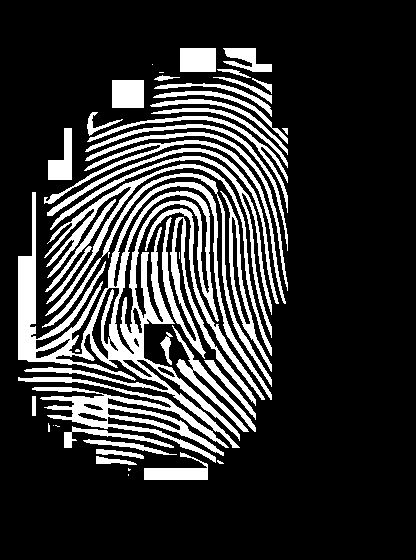
\includegraphics[width=\linewidth]{obrazky-figures/gabor_filtered_binarized.png}
      \caption{binarizovaná}
      \label{obr:gabor_binar}
    \end{subfigure}
    \hfill
    \begin{subfigure}[b]{0.3\linewidth}
      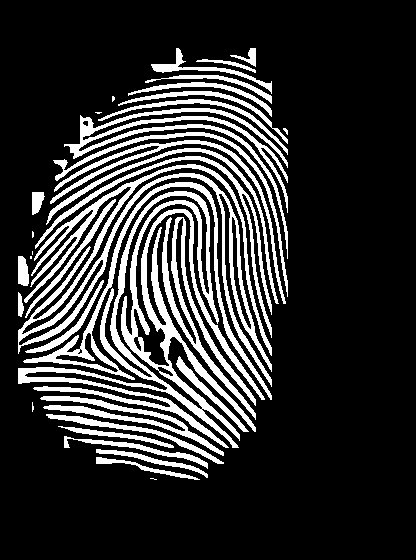
\includegraphics[width=\linewidth]{obrazky-figures/gabor_filtered_binarized_freq_blur.png}
      \caption{po rozostrení frekvencií}
      \label{obr:gabor_binar_freq_blur}
    \end{subfigure}
    \caption{Snímka odtlačku prsta filtrovaná Gabor filtrom (a), jej binarizovaná verzia (b) a~binarizovaná verzia po filtrovaní na základe rozostrenej
            frekvenčnej snímky (c).}
    \label{obr:gabor}
  \end{figure}

  \subsection{Stenčovanie línií}
  Vykonávané funkciou \texttt{zhangSuen}, stenčovanie sa vykonáva paralelnou metódou Zhang-Suen. Algoritmus je riadený hlavným cyklom, v rámci ktorého sú
  dva podcykly odstraňujúce pixely nepríslušiace kostre odtlačku prsta. Vstupom tejto funkcie je binarizovaná snímka získaná funkciou \texttt{gaborFilter}.
  Výstup tejto funkcie je binárna snímka stenčených papilárnych línií. Avšak výstupná snímka reprezentuje papilárne línie obrátene oproti predchádzajúcim
  krokom, a to tak, že línie sú reprezentované vyššími hodnotami, než pozadie snímky (viď obrázok~{\ref{obr:stencene}}), teda línie sú bledé na rozdiel od
  tmavých. Toto má význam pri nasledujúcich krokoch analýzy.

  \begin{figure}[h]
    \centering
    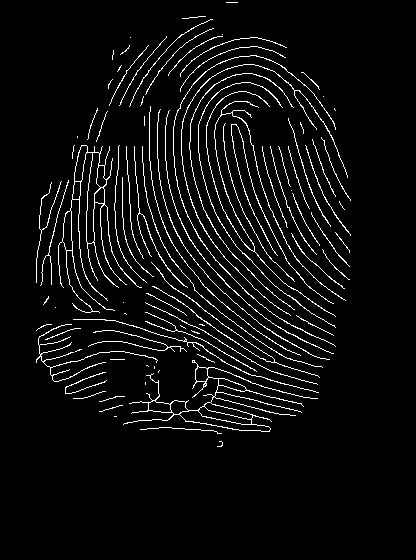
\includegraphics[width=0.3\linewidth]{obrazky-figures/thinned.png}
    \caption{Binárna snímka stenčených papilárnych línií.}
    \label{obr:stencene}
  \end{figure}

  \subsection{Markanty}
  Funkcia \texttt{extractMinutiae} prijíma binárnu snímku so stenčenými papilárnymi líniami. Každý pixel príslušný papilárnej línii je skontrolovaný
  maskami a pozícia vyhovjúcich pixelov je uložená do zvlášť dvojrozmerných polí. Oba kontrolované typy markantov (vidličky a ukončenia) sú ukladané do
  zvlášť polí, aby ich bolo možné separovať. Po extrakcii markantov funkcia vráti obe nové polia rovnakých veľkostí ako vstupná snímka. Tieto polia sú ďalej
  spracované funkciou \texttt{overlay}, ktorá vezme vstupnú snímku a dvojrozmerné pole rovnakej veľkosti s extrahovanými pozíciami markantov -
  v podstate maska pozícií. Následne sa na vstupnej snímke vyznačia oblasti špecifikované maskou, čím sa získa výstupná snímka, ktorá obsahuje značky na
  pozíciách extrahovaných markantov~(\ref{obr:markanty}).

  Extrahované markanty je možné následne exportovať do JSON súboru. Tento export sa vykonáva v metóde \texttt{exportMinutiaeJSON}, ktorá vezme pozície
  $xy$ jednotlivých extrahovaných markantov a orientáciu línií v danom pixeli a serializuje ich do JSON formátu. Výsledná serializovaná štruktúra markantov
  pozostáva z dvoch objektov (\uv{bifurcations} a~{\uv{ridgeEndings}}), ktoré obsahujú zoznam príslušných pozícií a orientácií línií. Je dôležité poznamenať,
  že do súboru sa ukladá orientácia papilárnych línií pod nájdeným markantom a nie orientácia samotného markantu.

  \begin{figure}[h]
    \centering
    \begin{subfigure}[b]{0.3\linewidth}
      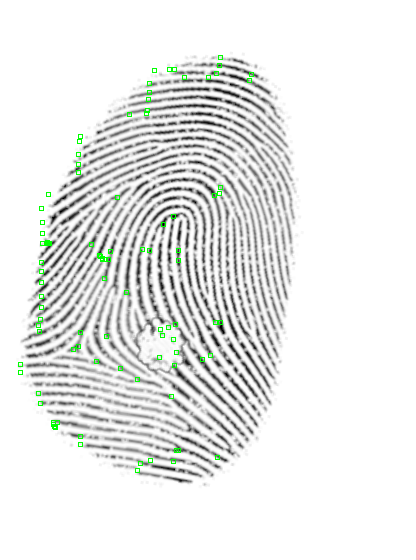
\includegraphics[width=\linewidth]{obrazky-figures/bifurcations.png}
      \caption{vidličky}
    \end{subfigure}
    \hspace{0.05\linewidth}
    \begin{subfigure}[b]{0.3\linewidth}
      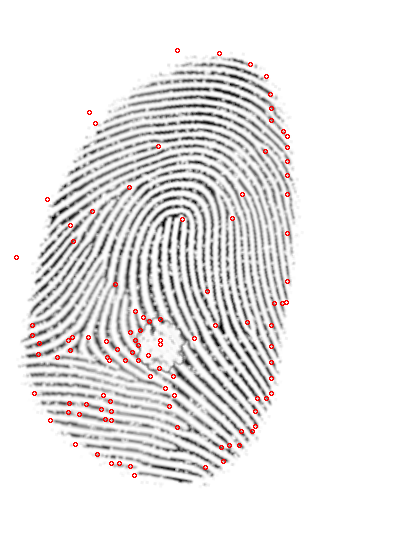
\includegraphics[width=\linewidth]{obrazky-figures/ridge_endings.png}
      \caption{ukončenia}
    \end{subfigure}
    \caption{Farebne vyznačené markanty na snímke odtlačku prsta.}
    \label{obr:markanty}
  \end{figure}

  \subsection{Singularity a triedy}
  Extrakcia singularít je riadená funkciou \texttt{poincare}, ktorá využíva metódu extrakcie Poincaré indexom. Funkcia prechádza každý pixel snímky orientácií
  a daný pixel spolu s jeho okamžitým okolím odovzdá funkcii \texttt{poincareIndex}. Tu sa okno, ktoré tvorí susedné pixely súčasného pixelu, cyklicky odvinie
  proti smeru hodinových ručičiek. Na odvinutom okne sa vypočíta Poincaré index pre daný pixel a táto hodnota sa vráti hlavnej riadiacej funkcii.
  V~závislosti hodnoty indexu sa jednotlivým snímkam singularít alebo jadier priradí príslušná hodnota - 1, ak sa jedná o singularitu, 0 inak.
  Výsledkom sú dve binárne snímky jadier a delt, ktoré majú vyznačené singularity v príslušných bodoch.
  
  Normalizácia snímok singularít sa vykonáva vo funkcii \texttt{singularityCleanup}. Táto funkcia plní dva účely. V prvom rade nahrádza oblasti s veľkým
  množstvom singularít rovnakého typu oblasťou s jednou singularitou umiestnenou na priemernú pozíciu detegovaných singularít v tejto oblasti.
  V druhom rade odstraňuje singularity rôzneho typu, ak sa nachádzajú v rovnakej oblasti. Výsledná snímka s detegovanými jadrami je zobrazená na
  obrázku~{\ref{obr:jadra}}, kde vyznačenie singularít prebehlo podobne ako pri markantoch pomocou funkcie \texttt{overlay}.

  \begin{figure}[h]
    \centering
    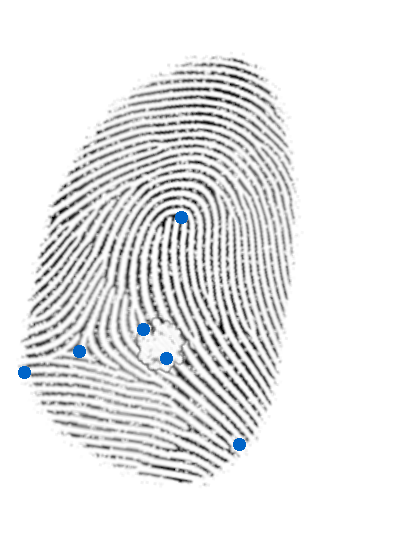
\includegraphics[width=0.3\linewidth]{obrazky-figures/cores.png}
    \caption{Snímka odtlačku prsta s vyznačenými detegovanými jadrami.}
    \label{obr:jadra}
  \end{figure}

  Detekciu triedy odtlačku prsta vykonáva funkcia \texttt{getClass}. Táto funkcia je schopná rozlíšiť oblúk, klenutý oblúk, ľavú slučku, pravú slučku.
  Špirálu a dvojitú slučku deteguje ako jednu triedu. Detekcia prebieha na základe pravidiel počtu singularít v jednotlivých triedach. V prípade, že sa
  v odtlačku nachádza po jednej z oboch singularít, rozlíšenie medzi klenutým oblúkom a slučkami sa vykoná na základe sklonu medzi singularitami.

  \section{Vyhodnotenie}
  Aplikácia je prevedená ako prenositeľná grafická pomôcka pre analýzu snímok odtlačkov prstov. Prenositeľnosť bola testovaná na zariadeniach s operačnými
  systémami Windows 10, macOS 10.15 a Debian 9.12 (stretch). Na všetkých systémoch bola aplikácia testovaná s rôznymi formátmi vstupných snímok. Medzi
  podporované formáty patria BMP, JPEG, PNG a WSQ a iné. Všetky súčasti aplikácie, až na jednu výnimku fungujú na všetkých testovaných systémoch. V prostredí
  Windows sa totiž počas testovania nepodarilo spojazdniť doplnkový modul \texttt{wsq} pre knižnicu Pillow.

  \subsection{Snímky rôznej kvality}
  V závislosti od kvality vstupnej snímky sa výsledky výstupov líšia. Toto je očakávané správanie, keďže vlastnosti odtlačku prsta zo snímky značne zlej
  kvality nie je možné spoľahlivo extrahovať. Je však nutné podotknúť, že kvalita spracovania snímky nie je vždy žiaduca aj v prípade kvalitnejšej vstupnej
  snímky. Tieto rozdiely je možné pozorovať na obrázku~{\ref{obr:porovnanie_kvality}}, kde sú zobrazené originálne snímky odtlačkov prstov rôznej kvality
  (avšak oba sú dostatočne vysokej kvality) a výstupy ich filtrovania Gabor filtrom a stenčenia línií. Je možné vidieť, že dopad na kvalitu filtrovania
  nemá výlučne iba ochorenie pokožky, ale aj nízky kontrast medzi papilárnymi líniami a pozadím - vidno na ľavej strane spodnej časti filtrovanej
  snímky~{\ref{obr:ecsema_gabor}}. Toto naznačuje nedostatočné alebo nekvalitné predspracovanie. Na týchto snímkach je tiež možné vidieť dopad prísneho
  prahovania pri vytváraní masky oblasti záujmu, čo sa prejavuje vo forme štvorcových fragmentov uprostred odtlačkov prstov.

  \begin{figure}[h]
    \centering
    \begin{subfigure}[b]{0.3\linewidth}
      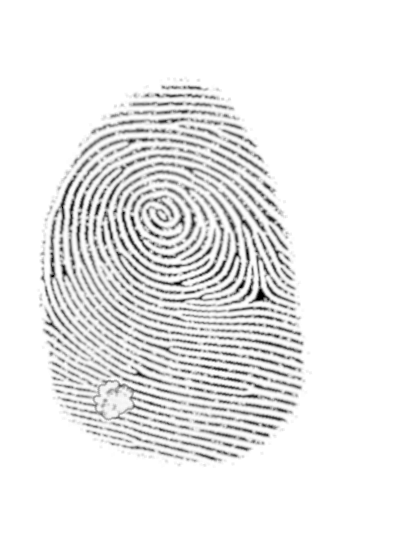
\includegraphics[width=\linewidth]{obrazky-figures/warts_orig.png}
      \caption{snímka vyššej kvality}
    \end{subfigure}
    \hfill
    \begin{subfigure}[b]{0.3\linewidth}
      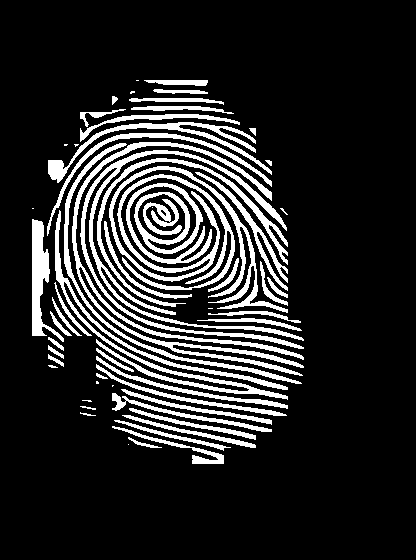
\includegraphics[width=\linewidth]{obrazky-figures/warts_gabor.png}
      \caption{filtrovaná Gabor filtrom}
    \end{subfigure}
    \hfill
    \begin{subfigure}[b]{0.3\linewidth}
      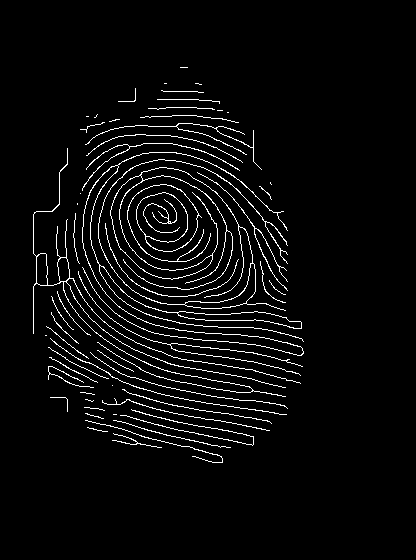
\includegraphics[width=\linewidth]{obrazky-figures/warts_thin.png}
      \caption{so stenčenými líniami}
    \end{subfigure}
    \\
    \begin{subfigure}[b]{0.3\linewidth}
      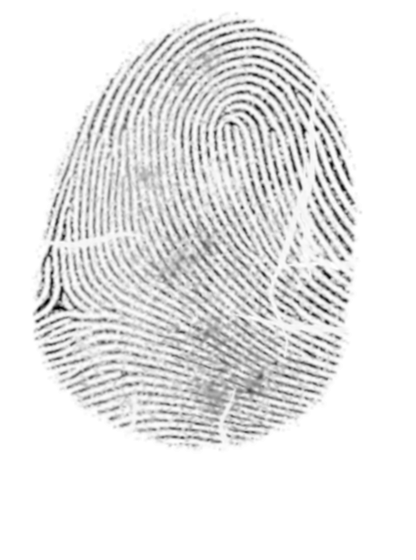
\includegraphics[width=\linewidth]{obrazky-figures/ecsema_orig.png}
      \caption{snímka nižšej kvality}
    \end{subfigure}
    \hfill
    \begin{subfigure}[b]{0.3\linewidth}
      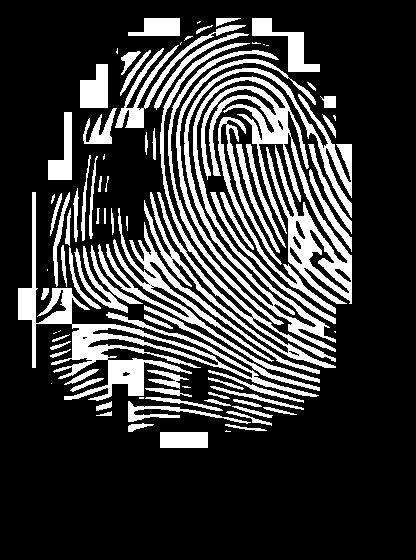
\includegraphics[width=\linewidth]{obrazky-figures/ecsema_gabor.png}
      \caption{filtrovaná Gabor filtrom}
      \label{obr:ecsema_gabor}
    \end{subfigure}
    \hfill
    \begin{subfigure}[b]{0.3\linewidth}
      \includegraphics[width=\linewidth]{obrazky-figures/ecsema_thin.png}
      \caption{so stenčenými líniami}
    \end{subfigure}
    \caption{Rozdiely v kvalite spracovania podľa rôznych kvalít vstupných snímok. Vo vrchnom riadku je možné vidieť snímku vysokej kvality a jej spracované
    verzie a v spodnom riadku je zobrazená snímka nižšej kvality. Snímky z internej databázy STRaDe.}
    \label{obr:porovnanie_kvality}
  \end{figure}

  Detekcia markantov prejavuje veľké množstvo falošných pozitívnych detekcií. Je však vhodné podotknúť, že samotná detekcia pracuje správne, avšak kroky
  predspracovania (obzvlášť Gabor filtrovanie a binarizácia) zavedú do binárnej snímky falošné markanty. V~dôsledku nedokonalého filtrovania a binarizácie
  sa vytvorí fragmentovaná snímka s veľkým množstvom falošných markantov v oblastiach ochorenia kože a prípadne iných oblastiach narušenia alebo meniacej
  sa frekvencie. Krok stenčovania línií produkuje kvalitné výsledky, na základe ktorých je možné spoľahlivo extrahovať markanty.

  Detekcia jadier nachádza jadrá okrem správnych miest aj na okrajoch oblasti záujmu kde orientácie prudko menia smer medzi oblasťou záujmu a pozadím snímky.
  Jedným z~možných riešení je opakované vyhladzovanie orientácií, kým sa nenájde platné množstvo singularít, ale z dôvodu pomalej implementácie algoritmu
  detekcie singularít bolo toto riešenie vypustené.
  Detekciu delt je možné považovať za nefunkčnú, pretože na testovacej vzorke niekoľkých desiatok snímok sa jej nepodarilo rozlíšiť ani jednu singularitu.
  Dopadom nefunkčnej detekcie singularít je nesprávna klasifikácia snímok do jednotlivých tried odtlačkov prstov.

  \subsection{Rýchlosť algoritmov}
  Knižnica \texttt{numpy} poskytuje možnosť využívania vektorizovaných operácií nad podporovanými dátovými typmi. Tieto operácie sú obecne veľmi rýchle
  a zároveň v prevedení \texttt{numpy} poskytujú intuitívne rozhranie pre ich aplikovanie. Nie všade je však možné využiť vektorizované operácie
  (aspoň nie intuitívne), čo často pri snímkach znamená implementáciu algoritmu pomocou cyklického prechádzania dátových polí snímky. V prípade interpretovaných
  jazykov ako Python to znamená značné spomalenie algoritmov. Rozdiel v rýchlosti vektorizovaných operácii oproti cyklickým riešením bol zjavný pri
  implementácií Gabor filtra, ktorý bol pôvodne plne cyklický. V takom prípade pri snímke veľkosti $400 \times 400$ trvala aplikácia filtra približne 70 sekúnd.
  Po vektorizovaní tvorby kernelu filtra sa algoritmus zrýchlil na približne 15 sekúnd. Ďalšie značné zrýchlenie by bolo možné dosiahnuť implementáciou
  algoritmov v kompilovanom jazyku (napr. C) alebo využitím C rozšírenia pre Python - Cython.

  %TODO mozno spravit tabulku s priemernou rychlostou jednotlvych algoritmov?
  %TODO dalsia subsekcia pre navrhy pre vylepsenia (napr. spojenie vizualizacie markantov do jedneho menu, namiesto do dvoch pre oba typy markantov)
  %LEFT-OFF-HERE

  \chapter{Záver}
  Táto práca bola zameraná na oboznámenie sa s odtlačkami prstov, rôznymi metódami ich snímania a krokmi ich spracovania a analýzy. Druhá kapitola poskytuje
  prehľad anatómie kože so zameraním na kožu na dlaniach a chodidlách, kde sa nachádzajú papilárne línie tvoriace odtlačky prstov. Ďalej sa venuje rôznym
  spôsobom zaznamenávania odtlačkov prstov ako sú rôzne typy snímačov a skenovanie daktyloskopických kariet. Sú tu uvedené aj spôsoby klasifikácie, spracovania
  a analýzy snímok odtlačkov prstov automatizovanými systémami. V tretej kapitole je popísaný rozšírený formát navrhnutý pre snímky odtlačkov prstov WSQ a jeho
  porovnanie s novším, ale obecnejším, formátom JPEG 2000. Predposledná kapitola je venovaná výstupu práce.

  Výstupom práce je aplikácia schopná predspracovať a analyzovať snímky odtlačkov prstov. Jedná sa o grafickú a prenositeľnú aplikáciu napísanú v jazyku
  Python. Podporuje veľké množstvo formátov snímok, medzi nimi aj formáty rozšírené v oblasti daktyloskopickej analýzy ako WSQ, JPEG 2000, PNG, BMP a iné.
  Aplikácia poskytuje možnosť vizualizácie jednotlivých zaužívaných krokov predspracovania snímok. Výsledky analýzy sú tiež zobrazené pomocou farebných
  značiek vrstvených na pôvodnú snímku. Cieľom týchto vizualizácií je demoštrácia úkonov spojených so spracovaním snímok pre ich lepšie pochopenie.
  Jednotlivé kroky spracovania snímok odtlačkov je možné exportovať do formátu špecifikovaného užívateľom.
  Užívateľ má tiež možnosť exportovať textový súbor obsahujúci popis extrahovaných markantov vo formáte JSON.

  Výsledná aplikácia však má priestor pre vylepšenie. Asi jej najvýraznejším nedostatkom je rýchlosť niektorých algoritmov, ktoré sa spoliehajú na
  cykly pre prácu s dátami snímok, pričom takáto implementácia v jazyku Python nie je ideálnym riešením. Prepísanie algoritmov do jazyka Cython by umožnilo
  zrýchlenie algoritmov, pričom by sa zachovala prenositeľnosť. Kvalita niektorých krokov spracovania tiež nie je vždy žiaduca, pretože so znižujúcou sa kvalitou
  vstupných snímok sa kvalita výstupov značne zhoršuje.

  Na záver by som rád dodal, že dúfam, že text tejto práce a jej výstup poskytne čitateľom pohľad do metód a procedúr využívaných v smere analýzy odtlačkov
  prstov.

  %\begin{figure}[]
  %  \centering
  %  % //TODO: nakreslit flowchart analýzy
  %  \includegraphics[width=5cm, height=5cm]{obrazky-figures/placeholder.pdf}
  %  \caption{Kroky automatického analyzátora}
  %  \label{obr:analysis_flowchart}
  %\end{figure}
